% Options for packages loaded elsewhere
\PassOptionsToPackage{unicode}{hyperref}
\PassOptionsToPackage{hyphens}{url}
\PassOptionsToPackage{dvipsnames,svgnames,x11names}{xcolor}
%
\documentclass[
]{interact}

\usepackage{amsmath,amssymb}
\usepackage{iftex}
\ifPDFTeX
  \usepackage[T1]{fontenc}
  \usepackage[utf8]{inputenc}
  \usepackage{textcomp} % provide euro and other symbols
\else % if luatex or xetex
  \usepackage{unicode-math}
  \defaultfontfeatures{Scale=MatchLowercase}
  \defaultfontfeatures[\rmfamily]{Ligatures=TeX,Scale=1}
\fi
\usepackage{lmodern}
\ifPDFTeX\else  
    % xetex/luatex font selection
\fi
% Use upquote if available, for straight quotes in verbatim environments
\IfFileExists{upquote.sty}{\usepackage{upquote}}{}
\IfFileExists{microtype.sty}{% use microtype if available
  \usepackage[]{microtype}
  \UseMicrotypeSet[protrusion]{basicmath} % disable protrusion for tt fonts
}{}
\makeatletter
\@ifundefined{KOMAClassName}{% if non-KOMA class
  \IfFileExists{parskip.sty}{%
    \usepackage{parskip}
  }{% else
    \setlength{\parindent}{0pt}
    \setlength{\parskip}{6pt plus 2pt minus 1pt}}
}{% if KOMA class
  \KOMAoptions{parskip=half}}
\makeatother
\usepackage{xcolor}
\setlength{\emergencystretch}{3em} % prevent overfull lines
\setcounter{secnumdepth}{5}
% Make \paragraph and \subparagraph free-standing
\ifx\paragraph\undefined\else
  \let\oldparagraph\paragraph
  \renewcommand{\paragraph}[1]{\oldparagraph{#1}\mbox{}}
\fi
\ifx\subparagraph\undefined\else
  \let\oldsubparagraph\subparagraph
  \renewcommand{\subparagraph}[1]{\oldsubparagraph{#1}\mbox{}}
\fi


\providecommand{\tightlist}{%
  \setlength{\itemsep}{0pt}\setlength{\parskip}{0pt}}\usepackage{longtable,booktabs,array}
\usepackage{calc} % for calculating minipage widths
% Correct order of tables after \paragraph or \subparagraph
\usepackage{etoolbox}
\makeatletter
\patchcmd\longtable{\par}{\if@noskipsec\mbox{}\fi\par}{}{}
\makeatother
% Allow footnotes in longtable head/foot
\IfFileExists{footnotehyper.sty}{\usepackage{footnotehyper}}{\usepackage{footnote}}
\makesavenoteenv{longtable}
\usepackage{graphicx}
\makeatletter
\def\maxwidth{\ifdim\Gin@nat@width>\linewidth\linewidth\else\Gin@nat@width\fi}
\def\maxheight{\ifdim\Gin@nat@height>\textheight\textheight\else\Gin@nat@height\fi}
\makeatother
% Scale images if necessary, so that they will not overflow the page
% margins by default, and it is still possible to overwrite the defaults
% using explicit options in \includegraphics[width, height, ...]{}
\setkeys{Gin}{width=\maxwidth,height=\maxheight,keepaspectratio}
% Set default figure placement to htbp
\makeatletter
\def\fps@figure{htbp}
\makeatother
% definitions for citeproc citations
\NewDocumentCommand\citeproctext{}{}
\NewDocumentCommand\citeproc{mm}{%
  \begingroup\def\citeproctext{#2}\cite{#1}\endgroup}
\makeatletter
 % allow citations to break across lines
 \let\@cite@ofmt\@firstofone
 % avoid brackets around text for \cite:
 \def\@biblabel#1{}
 \def\@cite#1#2{{#1\if@tempswa , #2\fi}}
\makeatother
\newlength{\cslhangindent}
\setlength{\cslhangindent}{1.5em}
\newlength{\csllabelwidth}
\setlength{\csllabelwidth}{3em}
\newenvironment{CSLReferences}[2] % #1 hanging-indent, #2 entry-spacing
 {\begin{list}{}{%
  \setlength{\itemindent}{0pt}
  \setlength{\leftmargin}{0pt}
  \setlength{\parsep}{0pt}
  % turn on hanging indent if param 1 is 1
  \ifodd #1
   \setlength{\leftmargin}{\cslhangindent}
   \setlength{\itemindent}{-1\cslhangindent}
  \fi
  % set entry spacing
  \setlength{\itemsep}{#2\baselineskip}}}
 {\end{list}}
\usepackage{calc}
\newcommand{\CSLBlock}[1]{\hfill\break\parbox[t]{\linewidth}{\strut\ignorespaces#1\strut}}
\newcommand{\CSLLeftMargin}[1]{\parbox[t]{\csllabelwidth}{\strut#1\strut}}
\newcommand{\CSLRightInline}[1]{\parbox[t]{\linewidth - \csllabelwidth}{\strut#1\strut}}
\newcommand{\CSLIndent}[1]{\hspace{\cslhangindent}#1}

\usepackage{booktabs}
\usepackage{longtable}
\usepackage{array}
\usepackage{multirow}
\usepackage{wrapfig}
\usepackage{float}
\usepackage{colortbl}
\usepackage{pdflscape}
\usepackage{tabu}
\usepackage{threeparttable}
\usepackage{threeparttablex}
\usepackage[normalem]{ulem}
\usepackage{makecell}
\usepackage{xcolor}
\usepackage{orcidlink}
\makeatletter
\@ifpackageloaded{caption}{}{\usepackage{caption}}
\AtBeginDocument{%
\ifdefined\contentsname
  \renewcommand*\contentsname{Table of contents}
\else
  \newcommand\contentsname{Table of contents}
\fi
\ifdefined\listfigurename
  \renewcommand*\listfigurename{List of Figures}
\else
  \newcommand\listfigurename{List of Figures}
\fi
\ifdefined\listtablename
  \renewcommand*\listtablename{List of Tables}
\else
  \newcommand\listtablename{List of Tables}
\fi
\ifdefined\figurename
  \renewcommand*\figurename{Figure}
\else
  \newcommand\figurename{Figure}
\fi
\ifdefined\tablename
  \renewcommand*\tablename{Table}
\else
  \newcommand\tablename{Table}
\fi
}
\@ifpackageloaded{float}{}{\usepackage{float}}
\floatstyle{ruled}
\@ifundefined{c@chapter}{\newfloat{codelisting}{h}{lop}}{\newfloat{codelisting}{h}{lop}[chapter]}
\floatname{codelisting}{Listing}
\newcommand*\listoflistings{\listof{codelisting}{List of Listings}}
\makeatother
\makeatletter
\makeatother
\makeatletter
\@ifpackageloaded{caption}{}{\usepackage{caption}}
\@ifpackageloaded{subcaption}{}{\usepackage{subcaption}}
\makeatother
\ifLuaTeX
  \usepackage{selnolig}  % disable illegal ligatures
\fi
\usepackage{bookmark}

\IfFileExists{xurl.sty}{\usepackage{xurl}}{} % add URL line breaks if available
\urlstyle{same} % disable monospaced font for URLs
\hypersetup{
  pdftitle={Quantile-parameterized distributions for expert knowledge elicitation},
  pdfauthor={Dmytro Perepolkin; Erik Lindström; Ullrika Sahlin},
  pdfkeywords={quantile functions, quantile-parameterized
distributions, expert knowledge elicitation, statistical distributions},
  colorlinks=true,
  linkcolor={blue},
  filecolor={Maroon},
  citecolor={Blue},
  urlcolor={Blue},
  pdfcreator={LaTeX via pandoc}}

\title{Quantile-parameterized distributions for expert knowledge
elicitation}
\author{Dmytro
Perepolkin$\textsuperscript{1}$~\orcidlink{0000-0003-2402-304X}, Erik
Lindström$\textsuperscript{2}$~\orcidlink{0000-0002-6468-2624}, Ullrika
Sahlin$\textsuperscript{1}$~\orcidlink{0000-0002-2932-6253}}

\thanks{CONTACT: Dmytro
Perepolkin. Email: \href{mailto:dmytro.perepolkin@cec.lu.se}{\nolinkurl{dmytro.perepolkin@cec.lu.se}}. Erik
Lindström. Email: \href{mailto:erik.lindstrom@matstat.lu.se}{\nolinkurl{erik.lindstrom@matstat.lu.se}}. Ullrika
Sahlin. Email: \href{mailto:ullrika.sahlin@cec.lu.se}{\nolinkurl{ullrika.sahlin@cec.lu.se}}. }
\begin{document}
\captionsetup{labelsep=space}
\maketitle
\textsuperscript{1} Centre for Environmental and Climate Science, Lund
University, Lund, Sweden\\ \textsuperscript{2} Centre for Mathematical
Sciences, Lund University, Lund, Sweden
\begin{keywords}
\def\sep{;\ }
quantile functions\sep quantile-parameterized distributions\sep expert
knowledge elicitation\sep 
statistical distributions
\end{keywords}

\section{Introduction}\label{introduction}

Judgment plays a crucial role in transforming raw data into meaningful
insights. To be useful, judgment must be translated into mathematical
models and assumptions. These models are designed to capture the
expert's understanding of the world, including the causal links between
relevant entities. The models serve as a representation of this
understanding, while also addressing knowledge limitations, treated as
uncertainties. Elicitation involves translating qualitative
understanding into quantitative models offering valuable insights.

\subsection*{Past research}\label{past-research}
\addcontentsline{toc}{subsection}{Past research}

Most of the expert elicitation protocols described in the literature
(Hanea et al. 2021; Gosling 2018; O'Hagan et al. 2006; Hemming et al.
2018; Morgan 2014; Welsh and Begg 2018; Spetzler and Staël Von Holstein
1975) encode expert judgments about the parameter or quantity of
interest as an ordered set of quantiles with corresponding
probabilities. This typically includes measures such as the median and
the upper and lower quartiles. Assessors are then encouraged to select a
probability distribution that reasonably fits the elicited
quantile-probability pairs and validate the choice with the expert
(Gosling 2018). A distribution is selected from a predefined set of
``simple and convenient'' distributions (O'Hagan et al. 2006) with
boundedness that accounts for the nature of the elicited quantity.

Several specialized distributions have been developed to facilitate
smooth interpolation of probabilistic assessments. These distributions,
parameterized by quantile-probability pairs, ensure that the elicited
quantile-probability pairs (QPPs) are exactly preserved (Keelin and
Powley 2011; Powley 2013; Keelin 2016; Christopher Campbell Hadlock
2017; Kevin J. Wilson et al. 2023). Quantile-parameterized distributions
are particularly valuable thanks to the interpretability of their
parameters. By leveraging the elicited quantiles, these distributions
enable precise capturing of expert knowlegde while maintaining a high
level of flexibility in modeling.

We believe that the primary utility of QPDs lies in their ability to
simplify the specification of probability distributions for model
parameters, known as \emph{prior elicitation} (Mikkola et al. 2021).
However, these same distributions can also be employed to describe an
expert's predictions for the next observation, referred to as
\emph{predictive elicitation} (Winkler 1980; J. B. Kadane 1980; Akbarov
2009; Hartmann et al. 2020), or to capture both uncertainty and
variability through a two-dimensional probability distribution in
\emph{hybrid elicitation} (Perepolkin, Goodrich, and Sahlin 2021).

This review paper aims to introduce quantile-parameterized distributions
(QPDs) to a wide readership. The literature review and the findings are
presented through the perspective of quantile functions, building upon
the theoretical foundations established by Parzen (Parzen 1979) and
Gilchrist (Gilchrist 2000). The derivatives and inverses for each of the
quantile functions discussed in the paper are provided in Appendix A,
serving as a valuable reference for future research. Through our
comprehensive review and identification of research gaps, we aim to
contribute to the development of flexible and extensible distributions
that can effectively capture expert knowledge. We hope that our overview
of quantile-parameterized distributions will be useful for researchers
and practitioners, enabling them to make an informed choice of a
distribution suitable for the task.

\subsection*{Paper structure}\label{paper-structure}
\addcontentsline{toc}{subsection}{Paper structure}

In Section 2, we revisit the approaches to quantile parameterization of
probability distributions and explore how QPDs can effectively describe
expert beliefs regarding model parameters or predictions. In Section 3,
we conduct a comprehensive review and comparison of various continuous
univariate QPDs found in the literature. Specifically, we focus on the
Myerson distribution and its generalization accommodating different tail
thicknesses. We compare the robust moments of QPDs to assess their
flexibility and behavior. This comparative analysis can guide the
selection of an appropriate distribution to characterize the quantity of
interest. In Section 4, we explore several methods for extending
univariate distributions to a multivariate setting. These methods
include the utilization of standard multivariate distributions (Drovandi
and Pettitt 2011), copulas (Hoff 2007), and bivariate quantiles (Nair
and Vineshkumar 2023; Vineshkumar and Nair 2019). We show how these
techniques can be applied to develop a bivariate version of the
Generalized Myerson distribution and demonstrate its application in
parametric and predictive elicitation. Finally, in Section 5, we discuss
future research directions and potential applications of QPDs in
Bayesian analysis.

\section{Quantile parameterization of probability
distributions}\label{quantile-parameterization-of-probability-distributions}

A fundamental principle in Bayesian data analysis is that learning from
data involves more than formulating hypotheses and models. It
necessitates articulating prior beliefs, expressing existing knowledge
mathematically, and translating it into probability distributions for
model parameters.

To accurately translate knowledge into the language of statistical
models the encoding distribution needs to be flexible, the process
should be transparent, and the results must be interpretable. For
continuous distributions, elicitation often consists of capturing a
series of quantile-probability pairs (QPPs) (J. Kadane and Wolfson 1998;
Morgan 2014), and then fitting a distribution to these pairs (O'Hagan
2019). However, in practice, the choice of a parametric distribution to
fit the elicited QPPs is often influenced by concerns about conjugacy
with the selected statistical model that represents the data-generative
process (the likelihood function) and/or the availability of required
distribution functions and fitting algorithms in the software employed.
Frequently, the selected distribution possesses fewer parameters than
the number of elicited QPPs, which can result in a less-than-perfect fit
(O'Hagan 2019). For instance, it is common to elicit three quantiles
(the median along with an upper and lower quartile) and subsequently
attempt to fit a normal or lognormal distribution (which features two
parameters) to these points.

An alternative approach to characterizing the distribution of
predictions or parameters is through quantile-parameterized
distributions (QPDs). These distributions are parameterized by the QPPs,
allowing the elicited values to directly define the distribution,
thereby ensuring a good fit and interpretability of parameters. The QPDs
examined in this paper can accommodate a wide range of shapes and
boundedness, making them valuable for accurately representing experts'
prior beliefs.

Parameterizing distributions using a vector of quantiles is not a novel
concept in the scientific community. The earliest mention can be traced
back to the \emph{substitution likelihood} proposed by Jeffreys
(Jeffreys 1939), which outlines a non-parametric procedure for inferring
the median using a set of sample quantiles. Subsequently, similar ideas
were further developed in (Boos and Monahan 1986; Lavine 1995; Dunson
and Taylor 2005).

All the QPDs found in the literature are constructed using the
\emph{quantile function}. These distributions are built either by
transforming simpler quantile functions or by simultaneous fitting of
parameterizing quantiles, as described below.

Let \(Y\) be a random variable with a (cumulative) distribution function
(CDF) denoted as \(F_Y(y\vert\theta)\). The quantile function (QF)
\(Q_Y(u\vert\theta)\) for \(Y\) is defined as

\[
Q_Y(u\vert\theta)=\inf\{y:F_Y(y\vert\theta)\geq u\}, \; u\in[0,1]
\]

Here, \(\theta\) represents the distribution parameter, and the
subscript \(_Y\) indicates that the depth \(u\) corresponds to the
random variable \(Y\).

Both the CDF and the QF are considered equally valid ways of defining a
distribution (Tukey 1965). For a quantile function that is
right-continuous and strictly increasing over the support of \(Y\), the
quantile function \(Q_Y(u)\) is simply the inverse of the distribution
function, denoted as \(Q_Y(u\vert\theta)=F_Y^{-1}(u\vert\theta)\).
Therefore, the quantile function is often referred to as the
\emph{inverse CDF}.

The derivative of the quantile function, known as the \emph{quantile
density function} (QDF), is denoted as \(q(u) = \frac{dQ(u)}{du}\). It
is reciprocally related to the probability density function (PDF)
\(f(x)\), such that \(f(Q(u))q(u) = 1\). The quantity
\(f_Y(Q_Y(u\vert\theta))=[q_Y(u\vert\theta)]^{-1}\) is referred to as
the \emph{density quantile} function (Parzen 1979) or \emph{p-pdf}
(Gilchrist 2000). The relationships between these functions are
concisely illustrated in the probability function Möbius strip
(Figure~\ref{fig-moebius-chart}).

\begin{figure}

\centering{

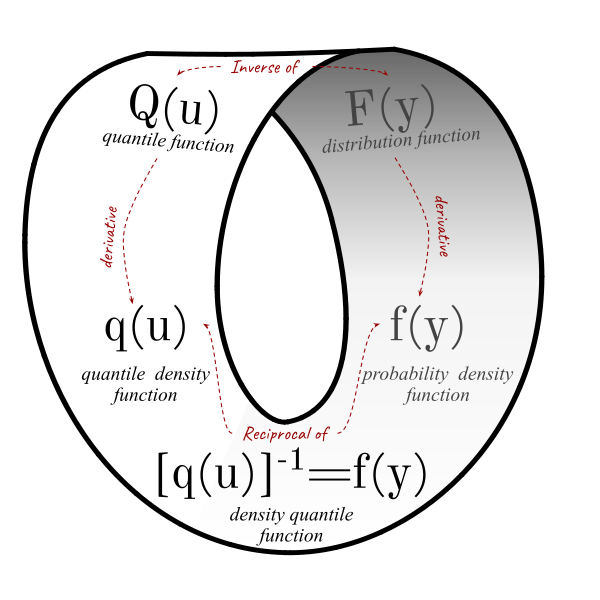
\includegraphics[width=0.4\textwidth,height=\textheight]{img/moebius-loop(1).png}

}

\caption{\label{fig-moebius-chart}Möbius strip of probability functions
(Perepolkin, Goodrich, and Sahlin 2023)}

\end{figure}%

Although many of the distributions discussed in Section 3 have
closed-form cumulative distribution functions (CDFs) and probability
density functions (PDFs), the functional form of the quantile function
(QF) is often simpler and can be reasoned about in terms of other
quantile functions, following \emph{Gilchrist's QF transformation rules}
summarized in Table~\ref{tbl-qf-trans}. This table presents the
addition, linear combination, and multiplication rules, which involve
two quantile functions \(Q_1\) and \(Q_2\). We will refer to these three
rules as \emph{Gilchrist combinations}, as they represent valid ways to
combine quantile functions to create new quantile functions.

\begin{table}

\caption{\label{tbl-qf-trans}Gilchrist's quantile function
transformation rules (Gilchrist 2000)}

\centering{

[ht]
\centering
\caption{\label{tab:tbl-qf-trans}}
\centering
\begin{tabular}[t]{l>{\raggedright\arraybackslash}p{3cm}>{\raggedright\arraybackslash}p{2.5cm}>{\raggedright\arraybackslash}p{3cm}}
\toprule
Original QF & Rule & Resulting QF & Resulting variable\\
\midrule
$Q_Y(u)$ & Reflection rule & $-Q(1-u)$ & QF of -Y\\
$Q_Y(u)$ & Reciprocal rule & $1/Q(1-u)$ & QF of $1/Y$\\
$Q_1(u), Q_2(u)$ & Addition rule & $Q_1(u)+Q_2(u)$ & valid QF\\
$Q_1(u), Q_2(u)$ & Linear combination rule & $aQ_1(u)+bQ_2(u)$ & valid QF for $a,b>0$\\
$Q_1(u),Q_2(u)>0$ & Multiplication rule & $Q_1(u)Q_2(u)$ & valid QF\\
\addlinespace
$Q_Y(u)$ & Q-transformation & $T(Q_Y(u))$ & QF of $T(Y)$,\newline  $T(Y)$ non-decreasing\\
$Q_Y(u)$ & p-transformation & $Q_Y(H(u))$ & p-transformation of $Q_Y(u)$,\newline  $H(u)$ non-decreasing\\
\bottomrule
\end{tabular}

}

\end{table}%

The quantile-parameterized distributions in this paper are categorized
into two groups based on their construction method. The first group
comprises distributions that are \emph{directly} parameterized by the
quantile-probability pairs (QPPs). This group includes the Myerson
distribution (Myerson 2005), and the Johnson Quantile-Parameterized
Distribution (Christopher C. Hadlock and Bickel 2017, 2019). These
distributions are constructed by reparameterizing or transforming
existing distributions, following Gilchrist rules
(Table~\ref{tbl-qf-trans}). The transformations used to construct them
are detailed in the next section.

The other group of distributions is \emph{indirectly} parameterized by
the QPPs. They require a fitting step where the quantile-probability
pairs are translated into distribution parameters, usually through
optimization or least-squares methods. This group includes the Simple
Q-Normal (Keelin and Powley 2011), Metalog (Keelin 2016), quantile
mixtures (Peng, Li, and Uryasev 2023), the variant of the Generalized
Lambda Distribution (GLD) by Chalabi et al (Chalabi, Scott, and Wuertz
2012), and the quantile-parameterized Triangular (Two-Sided Power)
distribution by Kotz and van Dorp (Kotz and Van Dorp 2004). Each
distribution's fitting method is described in the respective subsections
below.

\section{Univariate quantile-parameterized
distributions}\label{univariate-quantile-parameterized-distributions}

This section reviews various continuous univariate QPDs from the
literature. We then discuss the generalized form for these
distributions, based on the variations of these QPDs appearing in the
literature. For each distribution, we present its quantile function and
discuss the parameterization and feasibility conditions. The derivative
and inverse of each distribution can be found in Appendix A.

\subsection{Myerson distribution}\label{myerson-distribution}

One of the earliest examples of a distribution parameterized by
quantiles is the \emph{generalized log-normal} distribution defined by
the median and the upper and lower quartiles proposed by (Myerson 2005).
It relies on a transformation of the normal quantile function.

The Myerson distribution can be viewed as parameterized by three
quantile values \(\{q_1, q_2, q_3\}\), which correspond to the
cumulative probabilities \(\{\alpha, 0.5, 1-\alpha\}\). These quantiles
are symmetrical around the median and are defined by the tail parameter
\(0<\alpha<0.5\). This type of parameterization is known as the
Symmetric Percentile Triplet (SPT, \(\alpha\)-level SPT or
\(\alpha\)-SPT) and is also used in several other quantile-parameterized
distributions that we will describe below. The Myerson quantile function
is

\[
\begin{gathered}
\rho=q_3-q_2;\; 
\beta=\frac{\rho}{q_2-q_1};\;
\kappa(u)=\frac{S(u)}{S(1-\alpha)}\\
Q_Y(u \vert q_1,q_2,q_3,\alpha)=
\begin{cases}
q_2+\rho\frac{\beta^{\kappa(u)}-1}{\beta-1}, \quad &\beta \neq 1\\
q_2+\rho\kappa(u), \quad &\beta =1
\end{cases}
\end{gathered}
\]

Here, \(u\) represents the depth of the observations of the random
variable \(Y\) given the parameterizing \(\alpha\)-SPT
\(\{q_1, q_2, q_3, \alpha\}\), with \(0 < \alpha < 0.5\). The parameter
\(\rho\) is the \emph{upper p-difference}, and \(\beta\) is the ratio of
the inter-percentile ranges, known as the \emph{skewness ratio}
(Gilchrist 2000, 72). The \emph{kernel} quantile function \(S(u)\) is
equal to the quantile function of the standard normal distribution, also
referred to as the probit, defined as \(S(u) = \Phi^{-1}(u)\). The
formulas for the derivative and the inverse quantile function of the
Myerson QPD can be found in Appendix A.

It is important to note that while the Myerson distribution includes the
normal distribution as a special case when the skewness parameter
\(\beta = 1\), it can exhibit right-skewness or left-skewness for other
values of \(\beta\). In the symmetrical case, the range of the quantile
function is \((-\infty, \infty)\). For the right-skewed distribution
(\(\beta > 1\)), the range is
\((q_2 - \frac{\rho}{\beta - 1}, \infty)\), and for the left-skewed
distribution (\(0 < \beta < 1\)), the range is
\((-\infty, q_2 - \frac{\rho}{\beta - 1})\). The limiting case of the
skewed Myerson distribution \(\lim_{u \rightarrow 0} Q_Y(u\vert\theta)\)
for \(\beta > 1\) (and the other limit for \(0 < \beta < 1\)) possesses
some important properties that we discuss in
Section~\ref{sec-genmyerson} below.

The basic quantile function (Gilchrist 2000; Lampasi 2008) underlying
the Myerson distribution is a simple probit, \(S(u) = \Phi^{-1}(u)\),
transformed using the exponentiation function \(T(x) = \beta^{x}\),
where \(\beta > 0\) represents the skewness ratio (Gilchrist 2000). The
quantile parameterization is facilitated by \(\kappa(u)\), which takes
values \(\{-1,0,1\}\) for the three quantiles \(\{q_1, q_2, q_3\}\),
such that \(Q(\alpha) = q_1\), \(Q(0.5) = q_2\), and
\(Q(1 - \alpha) = q_3\).

\subsection{Johnson Quantile-Parameterized
Distribution}\label{johnson-quantile-parameterized-distribution}

Hadlock and Bickel (Christopher Campbell Hadlock 2017) reviewed the
existing quantile-parameterized distributions and proposed the quantile
parameterization of the Johnson SU family of distributions (N. L.
Johnson, Kotz, and Balakrishnan 1994). In their paper, Hadlock and
Bickel (Christopher C. Hadlock and Bickel 2017) presented two versions
of the distribution: the bounded (J-QPD-B) and the semi-bounded
(J-QPD-S), both parameterized by an SPT \(\{q_1, q_2, q_3, \alpha\}\)
and the bound(s).

The J-QPD-B distribution is obtained by applying the inverse-probit
transformation to the Johnson SU quantile function
\(Q_{SU}(u) = \xi + \lambda\sinh(\delta(S(u) + \gamma))\), where
\(\delta\) and \(\gamma\) are two shape parameters. This function is
then rescaled to the compact interval \([l_b, u_b]\). The J-QPD-B
quantile function is

\[
\begin{gathered}
Q_B(u\vert q_1, q_2, q_3, \alpha)=
\begin{cases}
l+(u_b-l_b)S^{-1}(\xi+\lambda\sinh(\delta(S(u)+nc))), \quad &n\neq0\\
l+(u_b-l_b)S^{-1}\left(B+\left(\frac{H-L}{2c}\right)S(u)\right), \quad &n=0
\end{cases}
\end{gathered}
\]

where

\[
\begin{gathered}
S(u)=\Phi^{-1}(u); \quad c=S(1-\alpha);\\
L=S\left(\frac{q_1-l_b}{u_b-l_b}\right); \quad  B=S\left(\frac{q_2-l_b}{u_b-l_b}\right);\\
H=S\left(\frac{q_3-l_b}{u_b-l_b}\right); \quad n=\text{sgn}(L+H-2B)\\
\xi=\begin{cases}L, \quad n=1,\\
B, \quad n=0,\\
H, \quad n=-1,\end{cases}\\
\delta=\frac{1}{c}\cosh^{-1}\left(\frac{H-L}{2\min(B-L,H-B)}\right)\\
\lambda=\frac{H-L}{\sinh(2\delta c)}
\end{gathered}
\]

\begin{figure}

\centering{

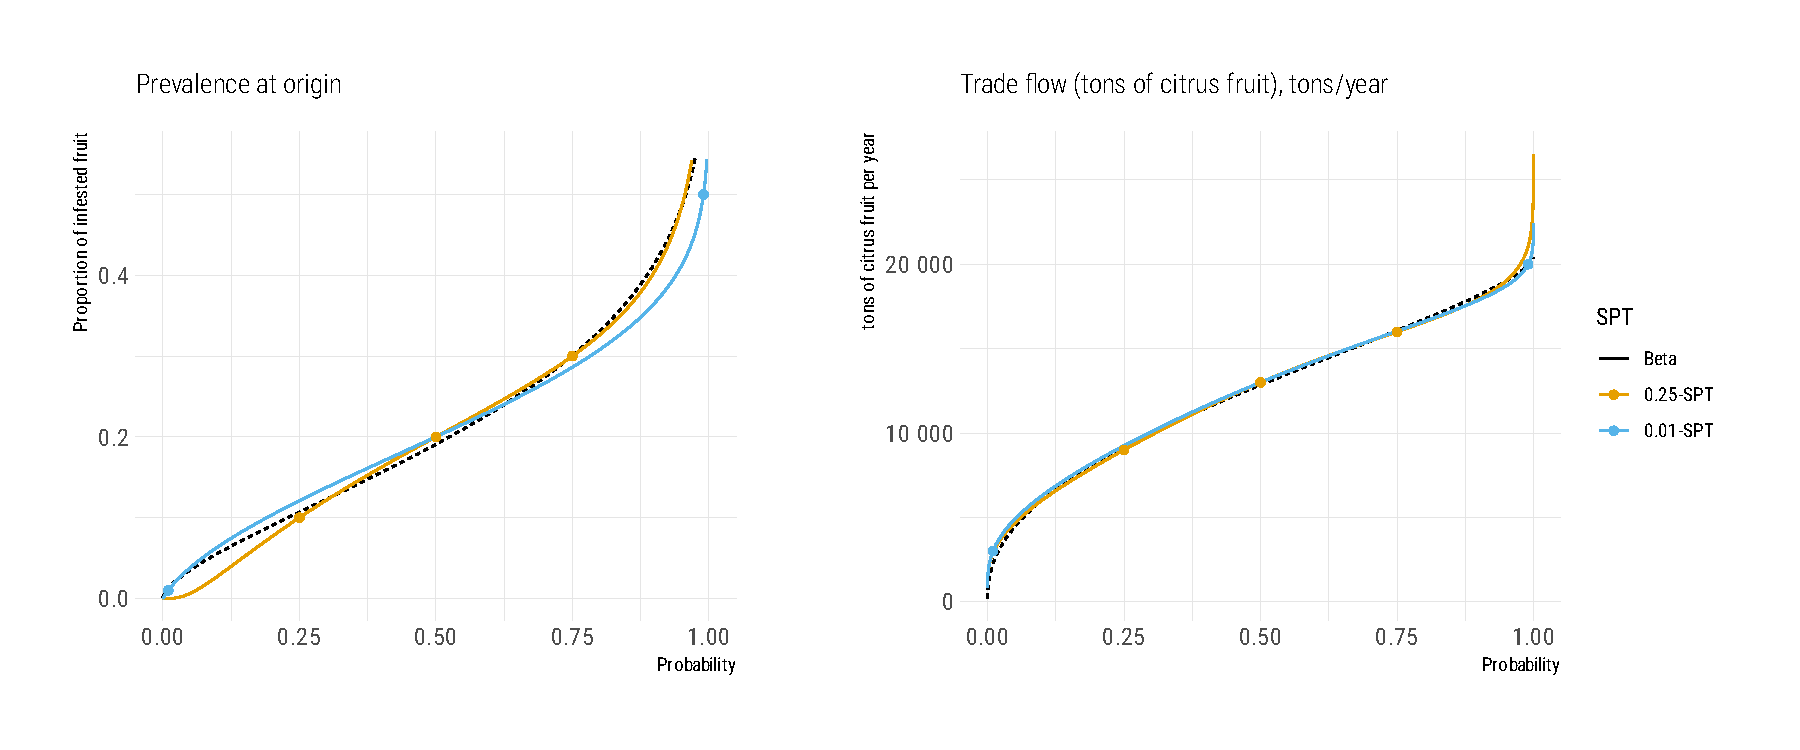
\includegraphics[width=1\textwidth,height=\textheight]{qpppp_files/figure-pdf/fig-jqpd1-1.pdf}

}

\caption{\label{fig-jqpd1}Fitted J-QPD-B (left) and J-QPD-S (right)
distribution for prevalence at origin and total trade flow,
respectively}

\end{figure}%

The left panel in Figure~\ref{fig-jqpd1} showcases the J-QPD-B quantile
function, which is parameterized using 0.25-SPT and 0.01-SPT assessments
of the proportion of fruit infested with \emph{Citripestis
sagittiferella}, as elicited by (EFSA et al. 2023). The dashed line
represents the Beta distribution fitted by the authors. The J-QPD-B,
being parameterized by an SPT, effectively captures three of the five
parameterizing quantiles, while the Beta distribution only provides an
approximation. Finding parameters of Beta distribution requires an
optimization step.

The J-QPD-S distribution is a semi-bounded variant of the distribution
that employs exponentiated hyperbolic arcsine transformations of the
Johnson's SU quantile function (Christopher C. Hadlock and Bickel 2017)

\[
\begin{gathered}
Q_S(u\vert q_1, q_2, q_3, \alpha)=\begin{cases}
l_b+\theta\exp\left(\lambda\sinh\left(\sinh^{-1}(\delta S(u))+\sinh^{-1}(nc\delta)\right)\right), \quad &n \neq 0\\
l_b+\theta\exp\left(\lambda\delta S(u)\right), \quad &n=0
\end{cases}
\end{gathered}
\]

where

\[
\begin{gathered}
S(u)=\Phi^{-1}(u); \quad c=S(1-\alpha);\\
L=\ln(q_1-l_b); \quad  B=\ln(q_2-l_b);\\
H=\ln(q_3-l_b); \quad n=\text{sgn}(L+H-2B)\\
\theta=\begin{cases}
q_1-l_b, \quad n=1,\\
q_2-l_b, \quad n=0,\\
q_3-l_b, \quad n=-1,\end{cases}\\
\delta=\frac{1}{c}\sinh\left(\cosh^{-1}\left(\frac{H-L}{2\min(B-L,H-B)}\right)\right)\\
\lambda=\frac{1}{\delta c}\min(H-B, B-L)
\end{gathered}
\]

When \(n=\text{sgn}(L+H-2B)\) evaluates to zero, he resulting
distribution is a lognormal distribution with parameters
\(\mu=\ln(\theta)=\ln(q_2-l_b)\) and \(\sigma=\lambda\delta=(H-B)/c\).
This distribution has support on the interval \([l_b,\infty]\).

The right panel in Figure~\ref{fig-jqpd1} depicts the J-QPD-S quantile
function, which is parameterized using 0.25-SPT and 0.01-SPT assessments
of the total trade flow for citrus fruit imported by the EU from
Indonesia, Malaysia, Thailand, and Vietnam in tons/year (EFSA et al.
2023).

\subsection{Generalisations of QPDs}\label{generalisations-of-qpds}

\subsubsection{Generalized Johnson Quantile-Parameterized
Distribution}\label{generalized-johnson-quantile-parameterized-distribution}

Hadlock and Bickel (Christopher C. Hadlock and Bickel 2019) introduced
the \emph{generalized} version of the Johnson Quantile-Parameterized
distribution system, denoted as G-QPD, by replacing the Normal
distribution in the core of the Johnson SU quantile function with the
quantile functions of the logistic and Cauchy distributions.

The generalized quantile function (QF) shares similarities with the
probit-based distribution described earlier, with \(S(u)\) defined as
the quantile function of either the logistic or Cauchy distribution.

The standard quantile function and distribution function of the logistic
distribution are given by:

\[
S(u)= \ln\left(\frac{u}{1-u}\right);\quad S^{-1}(y)=[\exp(-y)+1]^{-1}
\]

The standard quantile function and distribution function of the Cauchy
distribution are given by:

\[
S(u)= \tan\left[\pi\left(u-\frac{1}{2}\right)\right];\quad S^{-1}(y)=\frac{1}{ \pi}\arctan(y)+\frac{1}{2}
\]

Hadlock and Bickel (Christopher C. Hadlock and Bickel 2019) show that
the \emph{kernel} quantile function \(S(u)\) can be any standardized
(\(S(0.5)=0\)), symmetrical (\(s(u)=s(1-u)\)), and unbounded
(\(S(u)\in(-\infty;\infty)\)) quantile function with a smooth quantile
density \(dS(u)/du=s(u)\). The authors further showed that if \(S(u)\)
and \(S^{-1}(y)\) are expressible in closed-form, the quantile function
and distribution function of G-QPD will also be closed-form.

For the \emph{logistic} kernel, the G-QPD-S represents the generalized
log-logistic distribution, characterized by two shape parameters,
\(\lambda\) and \(\delta\). For the Cauchy kernel, the G-QPD-S
corresponds to the shifted log-Cauchy distribution (Christopher C.
Hadlock and Bickel 2019).

\subsubsection{Generalized Myerson distributions}\label{sec-genmyerson}

Following the approach in Hadlock and Bickel (Christopher C. Hadlock and
Bickel 2019), Myerson distribution can be generalized by substituting
the Normal kernel quantile function \(S(u)=\Phi^{-1}(u)\) with an
alternative symmetrical quantile function based on the depth \(u\).
Below, we discuss possible kernels and the resulting distributions:

\textbf{Logit-Myerson distribution}. Recently Wilson et al (Kevin J.
Wilson et al. 2023) reparameterized \emph{log-logistic distribution} in
terms of a Symmetric Percentile Triplet. Even though the authors do not
recognize it as such, the resulting quantile-parameterized distribution
is a Myerson distribution with logit kernel QF
\(S(u)=\ln\left(\frac{u}{1-u}\right)\)).

There could be several reasons why one might prefer the logit function
over the probit function (Berkson 1951). For example, distribution based
on logit may exhibit greater numerical stability due to its simple
closed-form quantile function, which does not rely on numerical
approximation during sampling. Logit-Myerson distribution displays
slightly heavier tails compared to the standard (probit-based) Myerson
distribution (Figure~\ref{fig-gmyerson-qfdqf-plot1}).

\textbf{Sech-Myerson distribution}. Following the same principle adopted
by Wilson et al. (Kevin J. Wilson et al. 2023) a variant of Myerson
distribution may be created using the hyperbolic secant quantile
function:

\[
S(u)=\ln\left[\tan\left(\frac{\pi}{2}u\right)\right]
\]

The Sech-Myerson distribution possesses thicker tails than the
Logit-Myerson distribution for the same parameterizing SPT
\(\{-5,4,16, 0.25\}\) (Figure~\ref{fig-gmyerson-qfdqf-plot1}). In
Section~\ref{sec-compareqf}, we conduct a comparative analysis of
different variations of the Generalized Myerson distribution alongside
their parametric counterparts and other quantile distributions.

\begin{figure}

\centering{

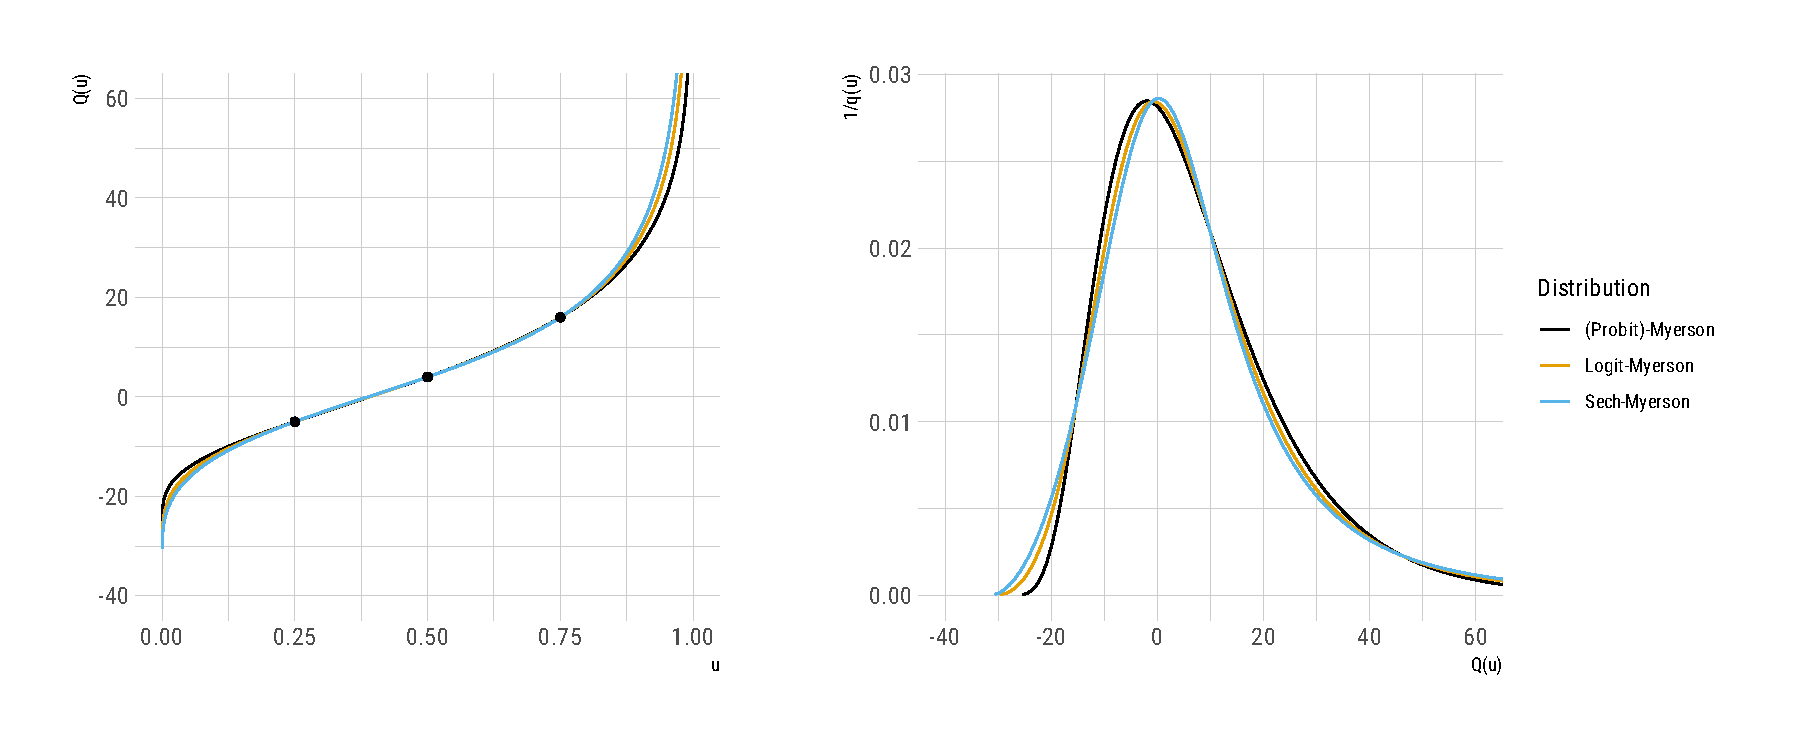
\includegraphics[width=1\textwidth,height=\textheight]{qpppp_files/figure-pdf/fig-gmyerson-qfdqf-plot1-1.pdf}

}

\caption{\label{fig-gmyerson-qfdqf-plot1}Quantile function and quantile
density of Generalized Myerson Distributions}

\end{figure}%

Theoretically, there is an infinite range of quantile function (QF)
kernels that can be utilized to generate new variations of the
Generalized Myerson distribution. These candidate kernel distributions
can even include shape parameters, as long as the resulting \(S(u)\)
remains standardized, symmetrical, and unbounded, as specified above.
For instance, it is possible to incorporate the basic QF of the Tukey
Lambda distribution \(S(u\vert\lambda)=u^\lambda-(1-u)^\lambda\) for a
fixed \(\lambda \neq 0\), or the Cauchy distribution
\(S(u)=\tan[\pi(u-0.5)]\), as employed by (Christopher C. Hadlock and
Bickel 2019). However, it is important to note that not all standard
quantile functions are created equal. To illustrate the issue of
unreliable kernels, let us consider Myerson distributions based on the
Cauchy and Tukey Lambda quantile functions (for \(\lambda=-0.5\)). As
can be observed in Figure~\ref{fig-gmyerson-qfdqf-plot2}, the density of
Generalized Myerson distribution with these kernels exhibits unexpected
spike near the lower bound.

\begin{figure}

\centering{

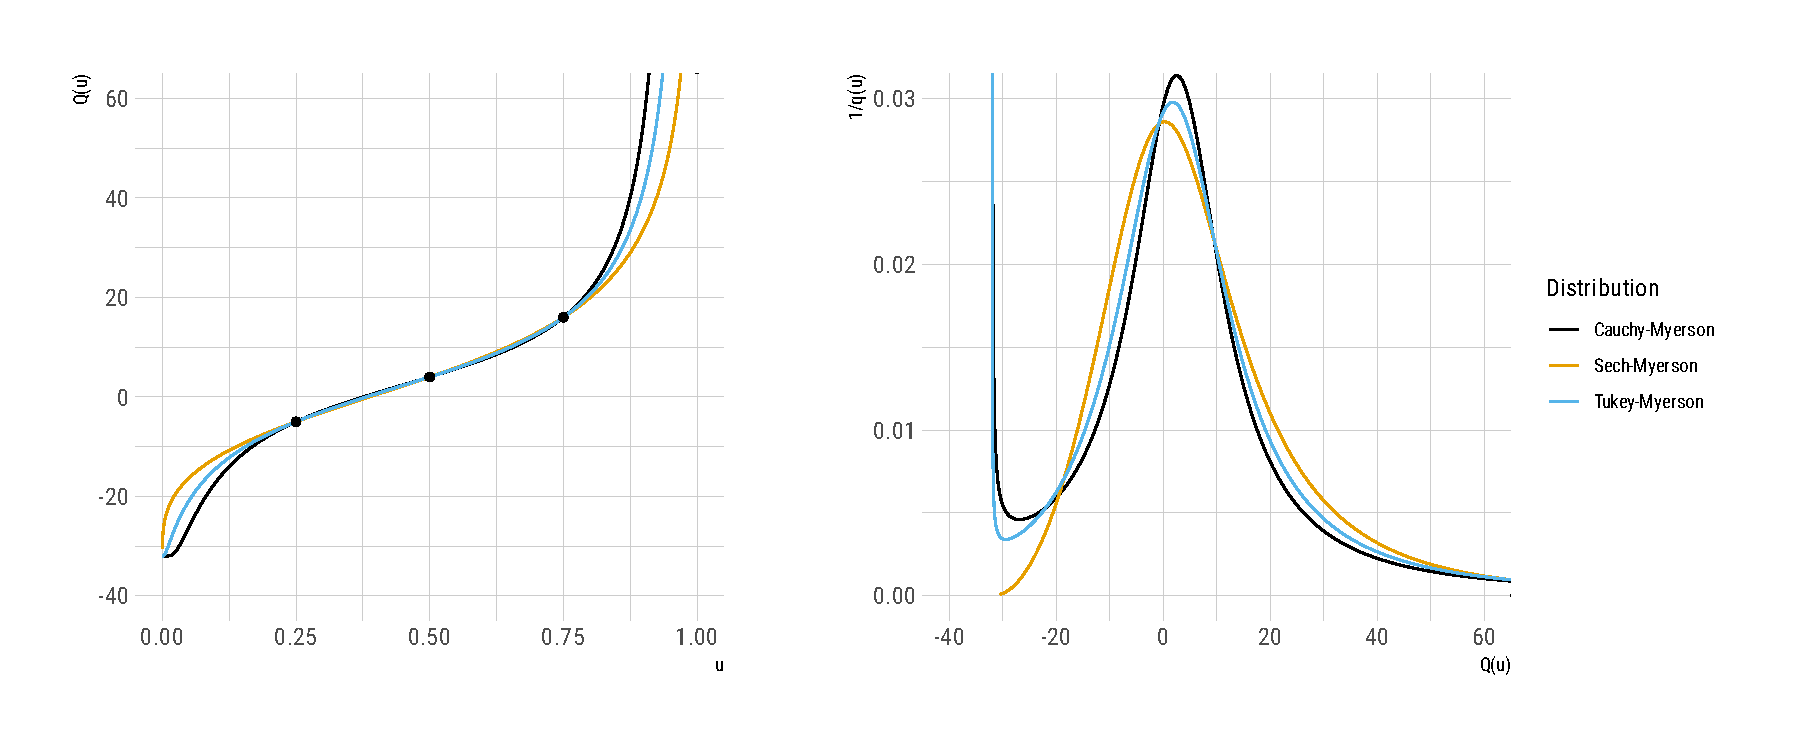
\includegraphics[width=1\textwidth,height=\textheight]{qpppp_files/figure-pdf/fig-gmyerson-qfdqf-plot2-1.pdf}

}

\caption{\label{fig-gmyerson-qfdqf-plot2}Quantile function and quantile
density of Generalized Myerson Distributions with unreliable kernels}

\end{figure}%

While all right-skewed Generalized Myerson distributions are bounded on
the left at
\(\lim_{u\rightarrow0}Q(u\vert\theta)=q_2-\rho\frac{1}{\beta-1}\)
regardless of the kernel used, the quantile density at the left limit
\(\lim_{u\rightarrow0}[q(u\vert\theta)]^{-1}\) is not independent of the
kernel. Although we can assume that \(q(0)=\infty\), the lower tail of
the density quantile function \([q(u)]^{-1}\) may exhibit a curling
effect for certain kernels, resulting in an increase in density for
lower values of \(u\). This effect is caused by the non-monotonic
behavior of the quantile convexity function \(c(u)=dq(u)/du\). This can
be easily verified by taking the second derivative of \(\beta^{S(u)}\)
for \(\beta>0\). While such kernels are mathematically valid and yield a
non-decreasing Generalized Myerson QF, we believe that they may be less
useful due to the counter-intuitive concentration of density in the
bounded tail. Consequently, we do not recommend using Cauchy or Tukey
Lambda kernels in practical applications.

\subsection{Simple Q-Normal, Metalog
distributions}\label{simple-q-normal-metalog-distributions}

An alternative system of quantile-parameterized distributions was
proposed by Keelin and Powley (Keelin and Powley 2011; Powley 2013).
This approach relies on the finite Taylor expansion of parameters in the
standardized quantile functions. Within this framework, two
distributions were introduced: the Simple Q-Normal distribution and the
Metalog distribution.

The Simple Q-Normal (SQN) distribution was developed by expanding the
parameters in the normal quantile function. Keelin et al.~(2011) used
this method to express the parameters of the normal quantile function
\(Q(u\vert\mu,\sigma)=\mu+\sigma z(u)\) as linear functions of the depth
\(u\). Specifically, \(\mu(u)=a_1+a_4u\) and \(\sigma(u)=a_2+a_3u\),
where \(z(u)=\Phi^{-1}(u)\) denotes the standard normal quantile
function. Therefore, the quantile function of the SQN distribution can
be expressed as follows:

\begin{equation}\phantomsection\label{eq-SQNQF}{
Q(u)= a_1+a_2z(u)+a_3uz(u)+a_4u\\
}\end{equation}

where \(z(u)=\Phi^{-1}(u)\), and \(a=\{a_1,a_2,a_3, a_4\}\) represents a
vector of parameters.

Consider a quantile-probability tuple of size 4, denoted as
\(\{\mathbf{p}, \mathbf{q}\}_4\), which consists of an ordered vector of
cumulative probabilities \(\mathbf{p}=\{p_1,p_2,p_3, p_4\}\) and an
ordered vector of corresponding quantiles
\(\mathbf{q}=\{q_1,q_2,q_3, q_4\}\). Substituting these vectors into the
SQN quantile function for \(u\) and \(Q(u)\), respectively, we obtain
the following matrix equation:

\begin{equation}\phantomsection\label{eq-sqn-matrix}{
\mathbf{q}=\mathbb Pa
}\end{equation}

where

\[
\begin{gathered}
\mathbb P=\begin{bmatrix} 1 & z(p_1) & p_1z(p_1) & p_1\\
                1 & z(p_2) & p_2z(p_2) & p_2\\
                1 & z(p_3) & p_3z(p_3) & p_3\\
                1 & z(p_4) & p_4z(p_4) & p_4\end{bmatrix}
\end{gathered}
\]

and \(a=\{a_1, a_2, a_3, a_4\}\) represents the parameter vector of the
SQN distribution.

The parameter vector \(a\) can be obtained by solving the matrix
Equation~\ref{eq-sqn-matrix}, given the 4-element quantile-probability
tuple \(\{\mathbf{p}, \mathbf{q}\}_4\) (Keelin and Powley 2011;
Perepolkin, Goodrich, and Sahlin 2021).

The same approach was later employed by (Keelin 2016) in creating the
metalog (meta-logistic) distribution. Starting with the quantile
function of the logistic distribution
\(Q(u\vert\mu,s)=\mu+s\text{logit}(u)\), where \(\mu\) corresponds to
the mean and \(s\) is proportional to the standard deviation
\(\sigma=s\pi/\sqrt3\), (Keelin 2016) expanded the parameters \(\mu\)
and \(s\) using a finite Taylor series centered at 0.5. Specifically,
\(\mu(u)=a_1+a_4(u-0.5)+a_5(u-0.5)^2+\dots\) and
\(s(u)=a_2+a_3(u-0.5)+a_6(u-0.5)^2+\dots\), where
\(a_i, \; i = \{1,2,\dots,n\}\) are real constants.

Therefore, the metalog quantile function is:

\[
Q(u)= a_1+a_2\text{logit}(u)+a_3(u-0.5)\text{logit}(u)+a_4(u-0.5)+a_5(u-0.5)^2\cdots,
\]

Given a QPT of size \(m\) denoted by \(\{\mathbf{p}, \mathbf{q}\}_m\),
where \(\mathbf{p}\) and \(\mathbf{q}\) are ordered vectors of
cumulative probabilities and corresponding quantiles, respectively, the
vector of coefficients \(\mathbf{a}={a_1,\dots,a_m}\) can be determined
by solving the matrix equation \(\mathbf{q}=\mathbb{P}\mathbf{a}\),
where \(\mathbf{p}\), \(\mathbf{q}\), and \(\mathbf{a}\) are column
vectors, and \(\mathbb{P}\) is an \(m \times n\) matrix:

\begin{equation}\phantomsection\label{eq-metalogPMatrixeq}{
\begin{gathered}
\mathbb{P} = \left[\begin{array}{lllll}
1  &\text{logit}(p_1) &(p_1-0.5)\text{logit}(p_1) &(p_1-0.5) &\cdots\\
1  &\text{logit}(p_2) &(p_2-0.5)\text{logit}(p_2) &(p_2-0.5) &\cdots\\
   &                  &\vdots\\
1  &\text{logit}(p_m) &(p_m-0.5)\text{logit}(p_m) &(p_m-0.5) &\cdots
\end{array}\right]
\end{gathered}
}\end{equation}

The vector of coefficients \(\mathbf{a}\) can be determined as
\(\mathbf{a}=[\mathbb{P}^{T}\mathbb{P}]^{-1}\mathbb{P}^{T}\mathbf{q}\).
If \(\mathbb{P}\) is a square matrix, meaning the number of terms \(n\)
is equal to the size of the parameterizing QPT \(m\), the equation can
be further simplified to \(\mathbf{a}=\mathbb{P}^{-1}\mathbf{q}\).
Metalog is said to be \emph{approximated} when the number of
quantile-probability pairs used for parameterization exceeds the number
of terms in the metalog QF (Keelin 2016; Perepolkin, Goodrich, and
Sahlin 2021).

The SQN and Metalog distributions are families of extended distributions
that, in theory, can have an arbitrary number of terms. Keelin (Keelin
2016) demonstrated the flexibility of the metalog distribution and its
ability to approximate arbitrarily complex probability density functions
with high precision, given enough terms in the metalog specification. In
practice, 10-15 terms are sufficient to approximate the distributional
shapes of virtually any complexity (Keelin and Howard 2021). Keelin
(Keelin 2016) introduced the bounded logit-metalog, the semi-bounded
log-metalog, and a special case of a 3-term metalog parameterized by
\(\alpha\)-SPT (SPT-metalog).

However, not all combinations of parameters \(\mathbf{a}\) in metalog
and SQN distributions result in a feasible (non-decreasing) quantile
function. For an arbitrary \(\mathbf{a}\)-vector, feasibility must be
checked (Keelin and Powley 2011). In the case of 3-term metalogs, the
feasibility conditions are straightforward (Keelin 2016). But as the
number of terms increases, such conditions become increasingly complex
(Keelin 2017). Having to deal with such feasibility requirements stands
in contrast with QF's that are constructed using Gilchrist rules
Table~\ref{tbl-qf-trans}, which guarantee feasibility.

\subsection{Quantile mixtures}\label{quantile-mixtures}

Recently (Peng, Li, and Uryasev 2023) proposed a novel framework for
extended quantile-parameterized distributions based on quantile mixtures
(not to be confused with CDF/PDF mixtures, (Gilchrist 2000, 107)). They
introduced a formulation in which a QPD quantile function is expressed
as a linear combination of \(I\) standardized quantile functions,
following Gilchrist's \emph{linear combination rule}
(Table~\ref{tbl-qf-trans}):

\[
G(u\vert\theta)=\sum_{i=0}^I\theta_iQ_i(u)
\]

Here, \(Q_i(u)\) represent basis quantile functions for the random
variable \(Y\) with \(Q_0(u)=1\), and
\(\pmb\theta=\{\theta_0,\theta_1,\dots,\theta_I\}\) is a non-negative
parameter vector that determines the contribution of each QF component
in the quantile mixture. To compute the coefficients \(\pmb\theta\), the
system of equations is solved

\[
\mathbf q=\mathbb Q \pmb\theta+\pmb\epsilon
\]

where \(\mathbf{q}=\{q_1,q_2,\dots, q_j\}\) is an ordered vector of
\(J\) parameterizing quantiles, corresponding to an ordered vector of
cumulative probabilities \(\mathbf{p}=\{p_1,p_2,\dots, p_j\}\),
\(\pmb\theta\) is a non-negative vector of \(I+1\) parameters,
\(\pmb\epsilon\) is a \(J\)-size vector of errors to be minimized, and
\(\mathbb Q\) is a \(J\times(I+1)\) matrix of regression factors

\[
\begin{gathered}
\mathbb{Q} = \left[\begin{array}{lllll}
1  &Q_1(p_1) &Q_2(p_1) &\cdots &Q_I(p_1)\\
1  &Q_1(p_2) &Q_2(p_2) &\cdots &Q_I(p_2)\\
   &\vdots   &\vdots   &\ddots \\
1  &Q_1(p_J) &Q_2(p_J) &\cdots &Q_I(p_J)
\end{array}\right]
\end{gathered}
\]

By ensuring non-negativity of weights (\(\theta_i\geq0\)), the solution
guarantees a proper non-decreasing quantile function. To estimate the
values of the vector \(\pmb\theta\in\Theta\), the authors suggest using
constrained weighted least squares regression with optional
regularization. The authors demonstrated that the estimator
\(\widehat{\pmb\theta}=\underset{\pmb\theta\in\Theta}{\text{argmin}} \left(\frac{1}{J}\sum_{j=1}^Jw_j\mathcal{E}_q(y_j-Q_j\pmb\theta)\right)^{\frac{1}{q}}\),
\(\mathcal{E}_q(x)=\lvert x \rvert^q\), \(w_j>0\), is asymptotically a
q-Wasserstein distance estimator, which converges in distribution to a
Normal distribution. The paper (Peng, Li, and Uryasev 2023) includes the
application of the quantile mixture model using a large number of
asymmetric t-distributions, and a quantile mixture of Generalized Beta
II distributions.

The quantile mixtures method of creating new QPDs guarantees feasibility
by construction, while affording nearly infinite flexibility, provided
that the component quantile functions are selected from a wide set of
distributions of varying shapes. Besides, a QPD constructed as a linear
combination of QFs is guaranteed to be unimodal, unless one of the
component in the mixture is multimodal (see Gilchrist 2000 for
examples). In addition, the method proposed by (Peng, Li, and Uryasev
2023) offers an advantage of resulting in closed-form quantile function
and quantile density function, provided that each of the components can
be expressed analytically. Unfortunately, neither asymmetric
t-distribution nor Generalized Beta II distribution, used by the
authors, has a closed-form QF. However, one can construct a highly
flexible quantile function using Gilchrist rules
(Table~\ref{tbl-qf-trans}) or use one of the existing well-studied QFs
discussed in the literature. In Section~\ref{sec-qmexample}, we provide
an example of using a quantile mixture of diversely-shaped quantile
functions to construct a bespoke highly flexible QPD.

\subsection{Other distributions}\label{other-distributions}

\subsubsection{Triangular and Two-Sided Power
distributions}\label{triangular-and-two-sided-power-distributions}

Several other distributions with at least some parameters mapped to
quantiles were proposed, including the reparameterization of the
Generalized Lambda Distribution by (Chalabi, Scott, and Wuertz 2012) and
the quantile-parameterized triangular (two-sided power) distribution by
(Kotz and Van Dorp 2004).

Kotz and van Dorp (Kotz and Van Dorp 2004) describe the
quantile-parameterized version of the triangular distribution (D.
Johnson 1997). This bounded distribution is widely used in the finance
and insurance industry and is popularized by the @Risk software package,
developed by Palisade (Palisade Corporation 2009). The triangular
distribution is parameterized by the two quantiles \(q_{a}\) and
\(q_{b}\), and the mode \(m\), subject to the constraint that
\(a\leq q_a\leq m\leq q_b\leq b\), where \(a\) and \(b\) represent the
lower and upper bounds, respectively. The standard quantile function for
the triangular distribution is expressed in terms of the bounds \(a\),
\(b\), and the mode \(m\).

\[
\begin{gathered}
Q(u\vert a,m,b)=\begin{cases}
a+\sqrt{u(m-a)(b-a)}, &\quad \text{for } 0\leq u \leq\frac{m-a}{b-a}\\
b-\sqrt{(1-u)(b-m)(b-a)}, &\quad \text{for } \frac{m-a}{b-a}\leq u \leq 1
\end{cases}
\end{gathered}
\]

In (Kotz and Van Dorp 2004) the authors show that given the two
parameterizing quantile-probability pairs \({q_a,p_a}\) and
\({q_b,p_b}\) and the mode value \(m\), there exists a unique value of
depth \(p_a<p<p_b\) corresponding to the root of the function

\[
g(p)=\frac{(m-q_a)(1-\sqrt{\frac{1-p_b}{1-p}})}{(q_b-m)(1-\sqrt{\frac{p_a}{p}})+(m-q_a)(1-\sqrt{\frac{1-p_b}{1-p}})}-p
\]

The root value \(p\in (p_a,p_b)\) of the function \(g(p)\) can be found
using any of the bracketing root-finding algorithms (Perepolkin,
Goodrich, and Sahlin 2023). It can then be substituted into the
following expressions to find the lower \(a\) and upper \(b\) limit
parameters of the triangular distribution:

\[
\begin{gathered}
a(p) \equiv \frac{q_a-m\sqrt{\frac{p_a}{p}}}{1-\sqrt{\frac{p_a}{p}}}, \quad a(p)<q_a\\
b(p) \equiv \frac{q_b-m\sqrt{\frac{1-p_b}{1-p}}}{1-\sqrt{\frac{1-p_b}{1-p}}}, \quad b(p)>q_b
\end{gathered}
\]

The book (Kotz and Van Dorp 2004) provides an algorithm for fitting a
four-parameter generalization of the triangular distribution called the
Two-Sided Power Distribution (TSP), using three quantile-probability
pairs and a mode value. For more information on fitting the
Quantile-Parameterized TSP Distribution by quantiles, refer to Section
4.3.3 of (Kotz and Van Dorp 2004).

\subsubsection{Generalized Lambda Distribution}\label{sec-gld}

Chalabi, Scott and Würtz (CSW) (Chalabi, Scott, and Wuertz 2012)
proposed an asymmetry-steepness reparameterization of the Generalized
Lambda Distribution (GLD) (Freimer et al. 1988) with four parameters.
This reparameterization involves mapping the location to the median and
the scale to the interquartile range (IQR), which corresponds to the
first and second robust moments (Kim and White 2004; Moors 1988).

The reparameterized Generalized Lambda Distribution (CSW GLD) has a
quantile function given by

\[
Q(u\vert\tilde\mu,\tilde\sigma,\chi,\xi)=\tilde\mu+\tilde\sigma\frac{S\left(u\vert\chi,\xi\right)-S\left(\frac{1}{2}\vert\chi,\xi\right)}{S\left(\frac{3}{4}\vert\chi,\xi\right)-S\left(\frac{1}{4}\vert\chi,\xi\right)}
\]

where \(\tilde\mu,\tilde\sigma,\chi,\xi\) represent the location, scale,
asymmetry, and steepness parameters, respectively. The specific form of
the basic function \(S(u)\) depends on the values of the parameters
\(\chi\) and \(\xi\)

\[
S(u\vert\chi,\xi)=
\begin{cases}
\begin{aligned}
&\ln(u)-\ln(1-u),  \quad \text{if }\chi=0,\xi=0.5&\\
&\ln(u)-\frac{1}{2\alpha}\left[(1-u)^{2\alpha}-1\right], \quad \text{if }\chi\neq0,\xi=\frac{1}{2}(1+\chi)&\\
&\frac{1}{2\beta}\left[u^{2\beta}-1\right]-\ln(1-u), \quad \text{if }\chi\neq0,\xi=\frac{1}{2}(1-\chi)&\\
&\frac{1}{\alpha+\beta}\left[u^{\alpha+\beta}-1\right]-\frac{1}{\alpha-\beta}\left[(1-u)^{\alpha-\beta}-1\right], \quad \text{otherwise}
\end{aligned}
\end{cases}
\]

where \(\alpha=0.5\frac{0.5-\xi}{\sqrt{\xi(1-\xi)}}\) and
\(\beta=0.5\frac{\chi}{\sqrt{1-\chi^2}}\). The bounds of the
distribution are given by

\[
\begin{gathered}
S(0\vert\chi,\xi)=\begin{cases}
\begin{aligned}
&-\frac{1}{\alpha+\beta},\quad &\text{if }\xi<\frac{1}{2}(1+\chi)\\
&-\infty, \quad &\text{otherwise}
\end{aligned}
\end{cases}\\
S(1\vert\chi,\xi)=\begin{cases}
\begin{aligned}
&\frac{1}{\alpha-\beta},\quad &\text{if }\xi<\frac{1}{2}(1-\chi)\\
&\infty, \quad &\text{otherwise}
\end{aligned}
\end{cases}
\end{gathered}
\]

The CSW GLD can have unbounded, bounded, and semi-bounded support,
accommodating a wide range of shapes, including unimodal, monotone,
U-shaped, and S-shaped densities (Chalabi, Scott, and Wuertz 2012).
Although the CSW GLD is not strictly parameterized by quantiles, the
mapping of the location and scale parameters to the median and IQR makes
it a suitable candidate for expert-informed distribution specification.

Several specialized methods have been developed for fitting the GLD to
samples (Karian and Dudewicz 2003). The parameterization of the CSW GLD
simplifies the fitting process because two of the four parameters can be
directly calculated from the sample: the location parameter is equal to
the sample median, and the scale parameter is equal to the interquartile
range. The remaining parameters can be estimated using various methods,
including robust moment matching, quantile matching, trimmed L-moments,
distributional least squares/absolutes, as well as maximum likelihood
estimation (Chalabi, Scott, and Wuertz 2012; Gilchrist 2000). The range
of feasible values for the steepness and asymmetry parameters can be
further reduced with the shape conditions specified in Section 3.5 of
(Chalabi, Scott, and Wuertz 2012).

Recently, (Dedduwakumara, Prendergast, and Staudte 2021) proposed a new
method of matching the shape of the GLD distribution to data using the
probability density quantile (pdQ) function (Staudte 2017). For the
quantile function \(Q(v), \; v\in [0,1]\) and the corresponding density
quantile function \(f(Q(v))=[q(v)]^{-1}\), the pdQ is defined as

\[
f^*(v)=\frac{f(Q(v))}{E\left[f(Q(v))\right]}
\]

The probability density quantile function is defined on the unit square
and is independent of the location and scale parameters.

Since integrating the GLD density quantile function is difficult,
(Staudte 2017, sec. 2.2), proposed using the kernel density method to
estimate the empirical QDF and, thus, an empirical pdQ for samples from
continuous distributions. Fitting the CSW GLD to a sample can be reduced
to finding the asymmetry and steepness parameters that minimize

\[
\underset{\chi,\xi}{\text{argmin}}\int_0^1\left[f^*(v, \chi, \xi)-f_{e}^*(v)\right]^2du
\]

where \(f^*(v,\chi,\xi)\) is the pdQ of the CSW GLD, and \(f^*_e(v)\) is
the empirical pdQ of the sample. The authors (Dedduwakumara,
Prendergast, and Staudte 2021) suggest approximating the integral by a
discrete set of depths \(v\), replacing the integral with a sum.

\subsection{Example}\label{sec-qmexample}

As an illustration of a faithful approximation of a large number of
quantile-probability pairs by QPD, we take 4000 posterior samples (4
chains of 1000 samples each) of one of the random intercepts in the
Eight Schools example model included in the \texttt{cmdstanr} package
(Gabry and Češnovar 2022) in R. The Eight Schools problem (Rubin 1981)
measuring the effectiveness of SAT coaching program in 8 US schools is
often used as an example model in introductory classes on Bayesian
Statistics. In \texttt{cmdstanr} it is modeled using a hierarchical
Bayesian model with normal priors for each of the 8 random intercepts
\texttt{theta}. However, due to the low number of posterior samples and
the heterogeneity in the data, the marginal posterior distributions of
the intercept parameters \texttt{theta} deviate from the Gaussian shape
in various ways (Figure~\ref{fig-school-thetas}).

An empirical distribution of posterior samples from a Bayesian model can
be viewed as a large number of quantile-probability pairs. Although it
is unlikely that such number of quantile-probability pairs could ever be
elicitable from an expert (in our case 4000), it could still be of
interest to approximate such marginal posterior distribution with a
highly flexible quantile function, e.g.~for the purpose of posterior
passing (Brand et al. 2019; Pritsker 2021). Closed-form QF expression
for the posterior margins would allow reusing it as a prior in a similar
model at a later stage. We discuss multivariate extension of this idea
in Section~\ref{sec-multivariateqpd}.

\begin{figure}

\centering{

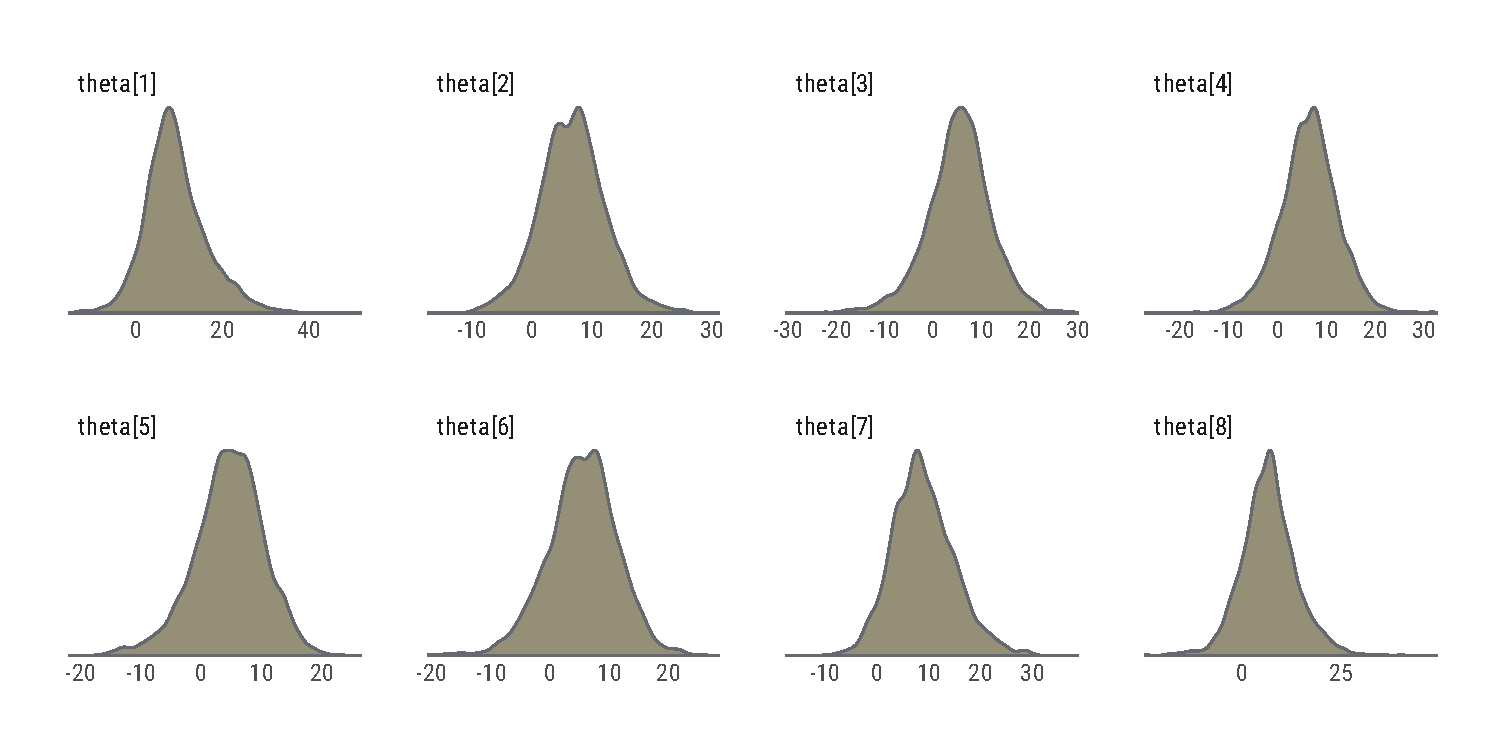
\includegraphics[width=1\textwidth,height=\textheight]{qpppp_files/figure-pdf/fig-school-thetas-1.pdf}

}

\caption{\label{fig-school-thetas}Posterior distributions of random
interecept parameters \texttt{theta} in the Eight Schools example model
(Gabry and Češnovar 2022)}

\end{figure}%

Figure~\ref{fig-fitted-qm} shows a QPD approximation of the marginal
distribution of \texttt{theta{[}5{]}} using a quantile mixture of
standardized (centered at zero and with the scale parameter set to one)
Chalabi, Scott, and Wuertz (2012) Generalized Lambda Distributions (CSW
GLD). In order to ensure the diversity of mixture components we
generated 400 independent uniformly distributed pairs of the two shape
parameters for GLD components using Hubbard (2019) pseudo random number
generator.

We constructed the matrix \(\mathbb Q\) above following the method
outlined by Peng, Li, and Uryasev (2023) and used Lawson-Hanson
non-negative least squares algorithm (implemented in \texttt{nnls}
package (Mullen and van Stokkum 2023) in R) to find the weights for each
of the mixture components. The non-zero elements are shows in
Figure~\ref{fig-gld-comp} along with the weights (which become the scale
parameters of the quantile mixture components).

\begin{figure}

\centering{

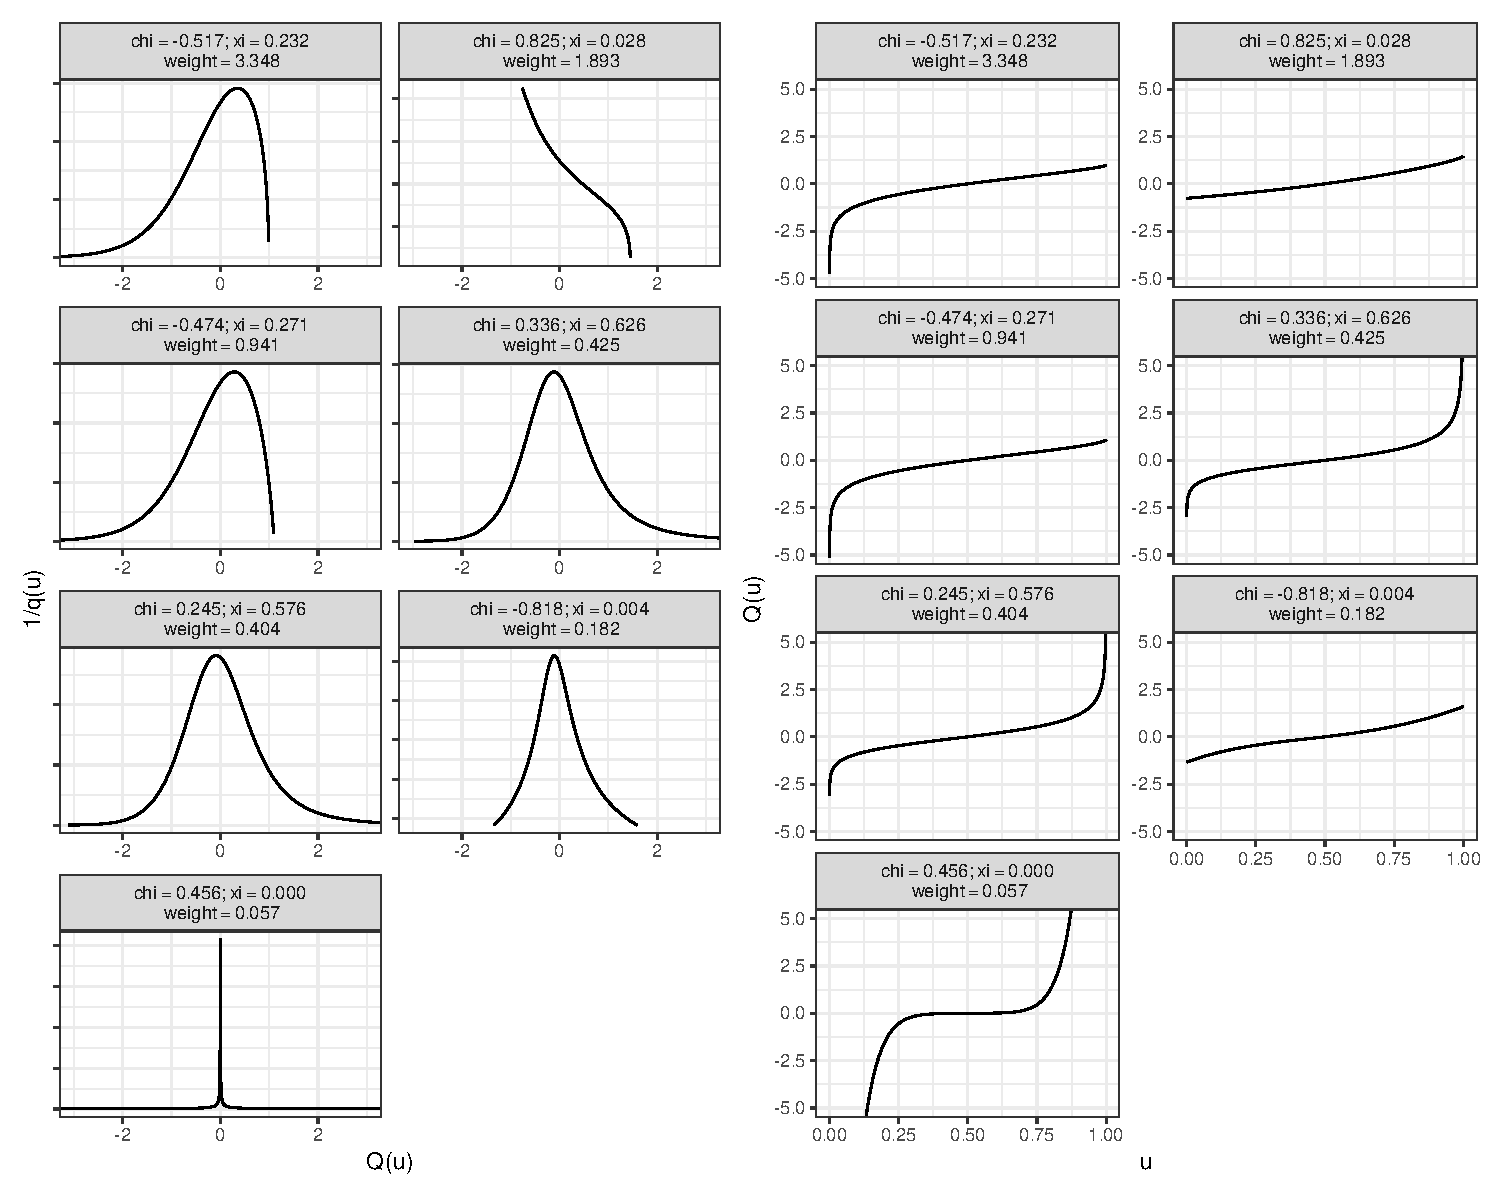
\includegraphics[width=1\textwidth,height=\textheight]{qpppp_files/figure-pdf/fig-gld-comp-1.pdf}

}

\caption{\label{fig-gld-comp}Density functions and quantile functions of
GLD components in approximating quantile mixture}

\end{figure}%

\begin{figure}

\centering{

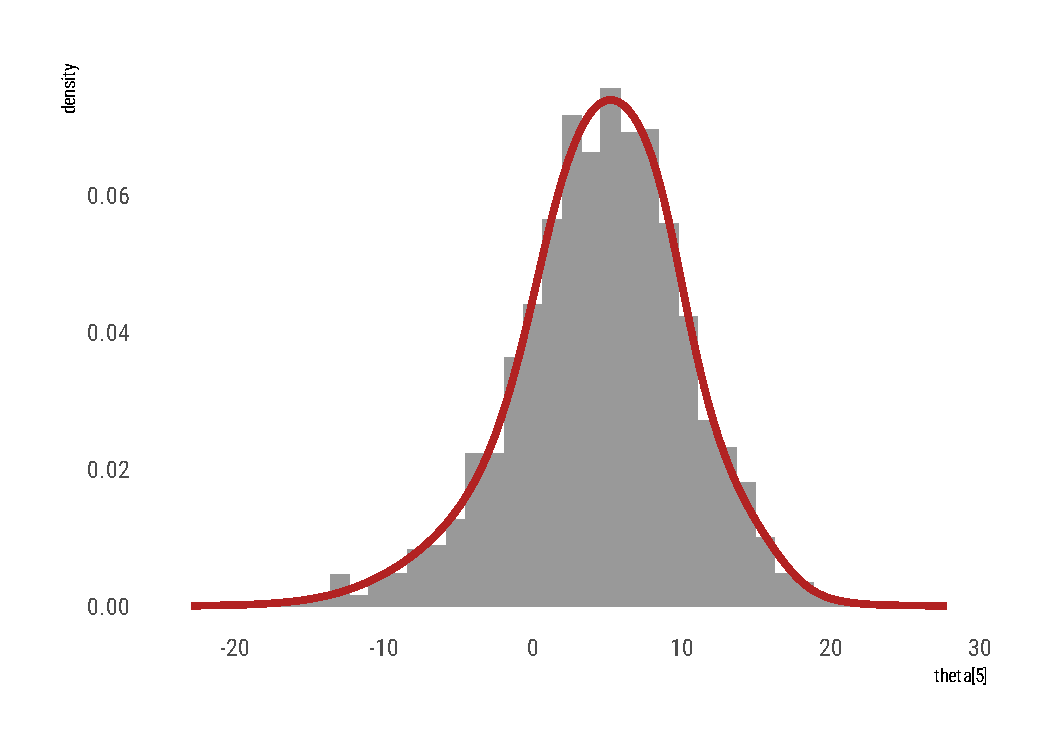
\includegraphics[width=0.8\textwidth,height=\textheight]{qpppp_files/figure-pdf/fig-fitted-qm-1.pdf}

}

\caption{\label{fig-fitted-qm}Distribution of posterior samples
approximated by the quantile mixture}

\end{figure}%

Figure~\ref{fig-fitted-qm} shows the histogram of 4000 parameter values
for \texttt{theta{[}5{]}} along with the approximation using the
quantile mixture with the components shown in Figure~\ref{fig-gld-comp}.
The resulting mixture is a linear combination of GLD quantile functions
with a closed form QF and DQF, which makes it possible to reuse this
distribution as a quantile-based prior in a Bayesian model (Perepolkin,
Goodrich, and Sahlin 2023).

\subsection{Choosing quantile-parameterized
distribution}\label{sec-compareqf}

A common approach to assess the properties of probability distributions
is through central moments, denoted by \(\mu_k=\mathbb{E}[(Y-\mu)^k]\),
where \(\mu\) represents the expected value of \(Y\). Karl Pearson
introduced a classification system for distributions using moment ratios
associated with skewness and kurtosis (Fiori and Zenga 2009):

\[
\beta_1=\frac{\mu_3^2}{\mu_2^3},\quad \beta_2=\frac{\mu_4}{\mu_2^2}
\]

While computing moments using the quantile function is straightforward
(the \(n\)-th raw moment is \(\mu_k=\int_0^1Q(u)^kdu\)), it may not be
possible to calculate higher-order moments for certain distributions.

Alternatively, robust alternatives to moments can be utilized, such as
the sample median \(\mu_r\), the interquartile range \(\sigma_r\), the
quartile-based robust coefficient of skewness \(s_r\) (Kim and White
2004), also known as Bowley's skewness (Bowley 1920) or Galton's
skewness (Gilchrist 2000), and the octile-based robust coefficient of
kurtosis \(\kappa_r\), also known as Moors' kurtosis (Moors 1988).

\[
\begin{aligned}
&\mu_r=Q(1/2)\\
&\sigma_r=Q(3/4)-Q(1/4)\\
&s_r=\frac{Q(3/4)+Q(1/4)-2Q(1/2)}{\sigma_r}\\
&\kappa_r=\frac{Q(7/8)-Q(5/8)+Q(3/8)-Q(1/8)}{\sigma_r}
\end{aligned}
\]

(Kim and White 2004; Arachchige, Prendergast, and Staudte 2022) have
proposed to standardize robust moments to facilitate their comparison
with the corresponding robust moments of the standard normal
distribution. (Groeneveld 1998; Jones, Rosco, and Pewsey 2011) have
introduced generalizations of robust moments to other quantiles.

Unlike moments, quantiles are always well defined, and since QPDs are
parameterized by quantile-probability pairs, quantile-based robust
moments can sometimes be directly computed from the parameters. For
instance, if the basic quantile function \(S(u)\) in
\(Q(u)=\mu+\sigma S(u)\) is standardized (such that \(S(0.5)=0\)), where
\(\mu\) and \(\sigma\) are the location and scale parameters of \(Q(u)\)
respectively, then \(\mu_r=\mu\). Moreover, \(\sigma_r\) is always
independent of location, and \(s_r\) and \(\kappa_r\) are independent of
both location and scale.

Figure~\ref{fig-unbounded}, Figure~\ref{fig-semibounded}, and
Figure~\ref{fig-bounded} resemble the Cullen and Frey (Cullen, Frey, and
Frey 1999) plots (Pearson plots), but instead of using central moments,
they employ quartile/octile-based robust metrics of skewness \(s_r\) and
kurtosis \(\kappa_r\) to compare the quantile-parameterized
distributions to some of their parametric counterparts.

In these plots, Metalog3 and Metalog4 refer to 3- and 4-term metalog
distributions, respectively, and GLDcsw refers to Chalabi et al
(Chalabi, Scott, and Wuertz 2012) parameterization of GLD. As can be
seen in Figure~\ref{fig-unbounded}, all generalizations of Myerson
distributions have higher robust kurtosis for the same robust skewness.
Additionally, GLD CSW is more flexible than the unbounded 4-term
metalog. The \emph{log}-transformed metalog distribution appears to be
the best among the semi-bounded distributions
(Figure~\ref{fig-semibounded}). Furthermore, the flexibility of the
bounded J-QPD-B is at least as good as that of the Beta and Kumaraswamy
distributions (Figure~\ref{fig-bounded}).

\begin{figure}

\centering{

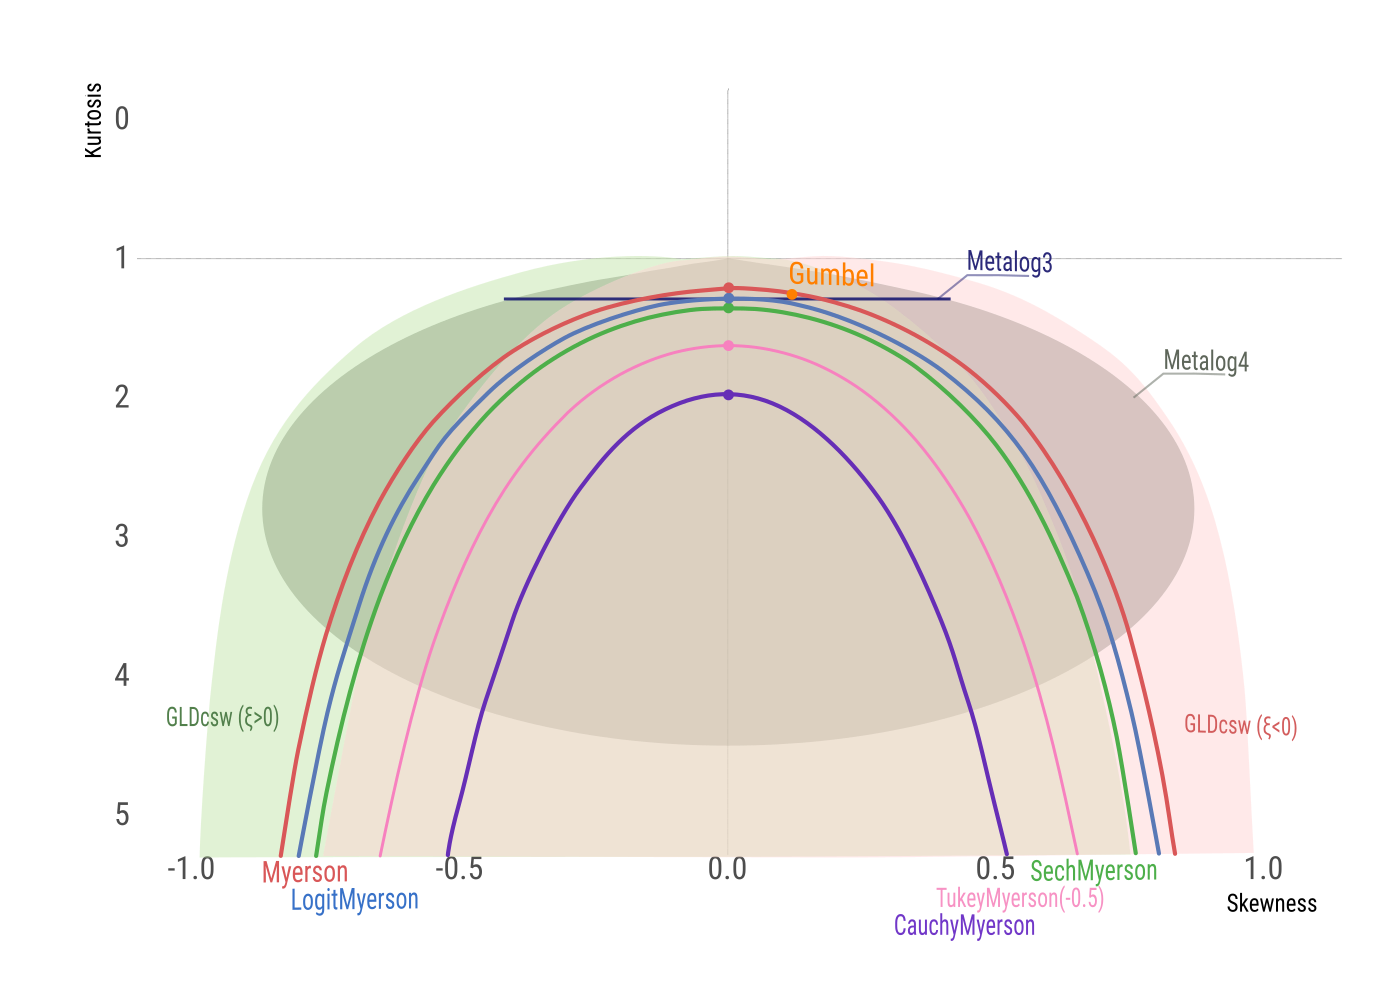
\includegraphics[width=0.8\textwidth,height=\textheight]{img/unbounded_final.png}

}

\caption{\label{fig-unbounded}Robust skewness vs robust kurtosis for
some unbounded distributions}

\end{figure}%

\begin{figure}

\centering{

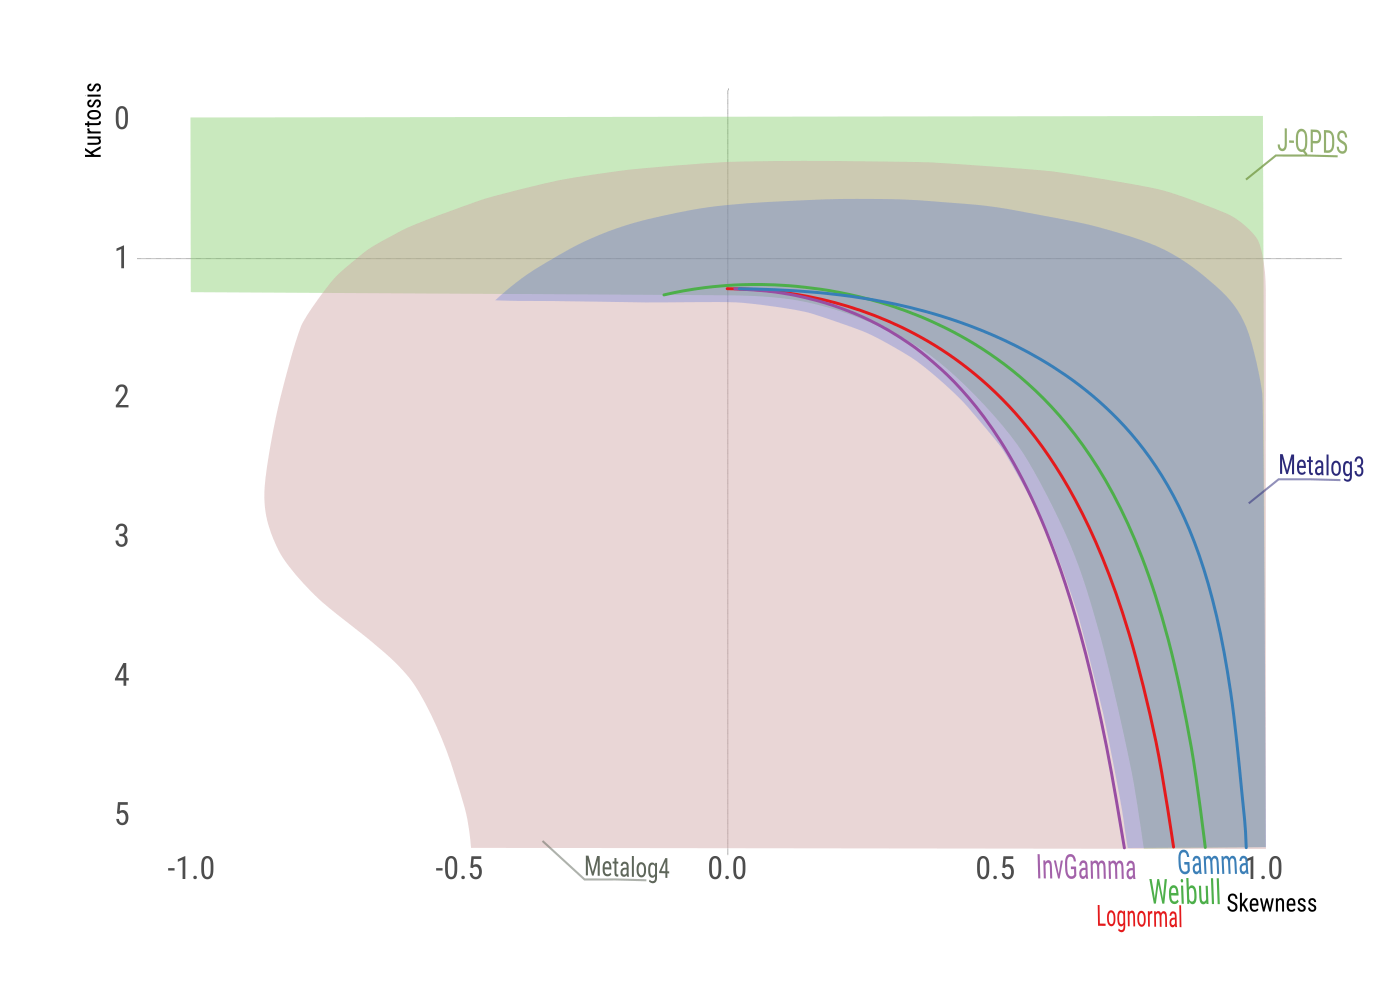
\includegraphics[width=0.8\textwidth,height=\textheight]{img/semibounded_final.png}

}

\caption{\label{fig-semibounded}Robust skewness vs robust kurtosis for
some left-bounded distributions}

\end{figure}%

\begin{figure}

\centering{

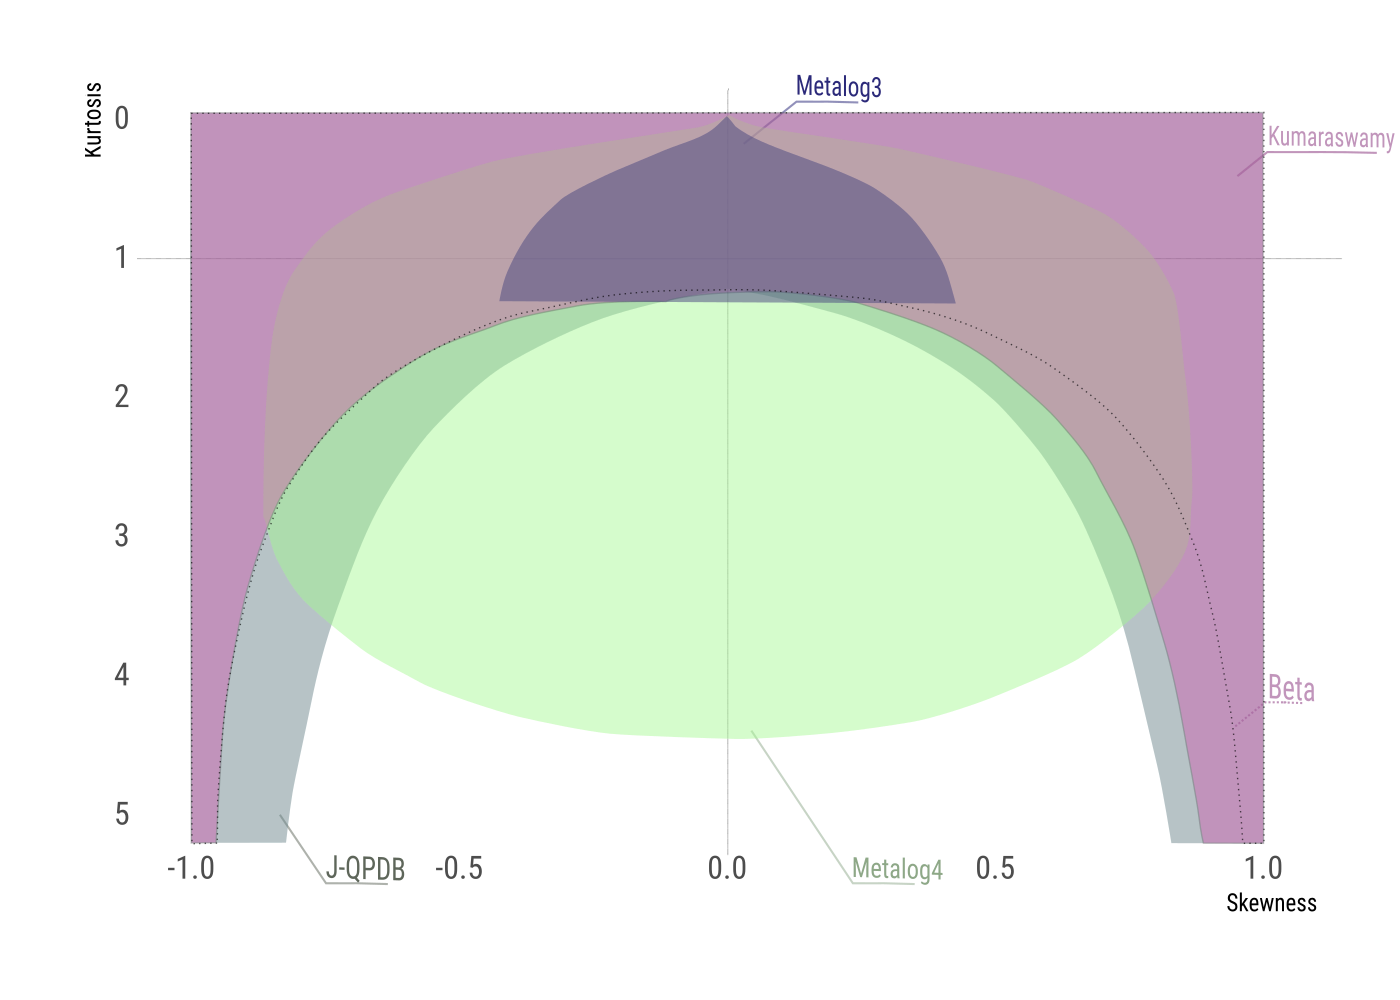
\includegraphics[width=0.8\textwidth,height=\textheight]{img/bounded_final.png}

}

\caption{\label{fig-bounded}Robust skewness vs robust kurtosis for some
bounded distributions}

\end{figure}%

\section{Multivariate quantile-parameterized
distributions}\label{sec-multivariateqpd}

Quantile-parameterized distributions can serve as marginal distributions
in multivariate models, where the dependency structure is captured by a
standard (parametric) multivariate distribution, a copula, or described
by bivariate quantiles. However, the marginal distributions alone are
insufficient to determine the corresponding bivariate distribution,
resulting in an infinite number of bivariate distributions with the same
margins (Gumbel 1960, 1961). In this section, we describe several
methods for extending the distributions parameterized by the
quantile-probability pairs to become Multivariate Quantile-Parameterized
Distributions (MQPDs).

\subsection{MQPDs based on standard multivariate
distributions}\label{mqpds-based-on-standard-multivariate-distributions}

\subsubsection{Normal distribution}\label{normal-distribution}

In the simplest case, multivariate Quantile-Parameterized Distributions
(MQPDs) can be created by using the multivariate normal distribution,
following the approach of (Hoff 2007). The Myerson, J-QPD, and SQN
quantile functions are Q-transformations of the probit
\(Q(z(u)\vert\theta)\), where \(z(u)=\Phi^{-1}(u)\) represents the
standard normal quantile function. The multivariate versions of these
distributions can be viewed as the Q-transformations of the multivariate
normal distribution. To extend these QPDs to \(J\) dimensions using the
multivariate normal distribution, we employ the method outlined in
(Drovandi and Pettitt 2011).

The \(i\)-th component of a single observation \(y_i\) can be described
by the quantile function:

\[
y_i=Q(z(u_i)\vert\theta_i), \; \text{for }i=1,\dots,J 
\]

where \(\theta_i\) represents the set of parameters for component \(i\)
(e.g., \(\{q_1,q_2,q_3, \alpha\}_i)\) for Myerson or J-QPD
distributions). The vector \((z(u_1),\dots,z(u_j))^T\sim N(0,\Sigma)\),
where \(\Sigma\) denotes the covariance matrix.

For invertible distributions, the inverse quantile function is the
cumulative distribution function (CDF)
\(Q^{-1}(y_i\vert\theta)=F(y_i\vert\theta)\), otherwise, the inverse can
be computed numerically as
\(\widehat{F}(y_i\vert\theta)=\widehat{Q^{-1}}(y_i\vert\theta)\)
(Perepolkin, Goodrich, and Sahlin 2023).

Drovandi and Pettitt (Drovandi and Pettitt 2011) show that the joint
density of a single (multivariate) observation \((y_i,\dots,y_J)\) can
be expressed as:

\[
f(y_1,\dots,y_J\vert\theta)=\varphi(z(Q^{-1}(y_1\vert\theta_1)),\dots,z(Q^{-1}(y_J\vert\theta_J));\Sigma)\prod_{i=1}^{J}\frac{dQ^{-1}(y_i\vert\theta_i)}{dy_i}
\]

where \(z(Q^{-1}(y_i\vert\theta_i))=z_i\),
\(\varphi(z_1,\dots,z_J;\Sigma)\) represents the multivariate normal
density with a mean of zero and a covariance matrix of \(\Sigma\), and
\(\frac{dQ^{-1}(y_i)}{dy_i}=f(y_i)\) is the probability density function
(PDF) of the QPD (refer to Appendix A).

For distributions without a PDF, the same joint density can be expressed
as a joint density quantile function

\[
[q(u_1,\dots,u_j)]^{-1}=\varphi(z(u_1),\dots,z(u_J);\Sigma)\prod_{i=1}^{J}[q(u_i\vert\theta_i)]^{-1}
\]

since \(Q^{-1}(y_i\vert\theta_i)=u_i\) and
\(f(y_i\vert\theta_i)=[q(u_i\vert\theta_i)]^{-1}\) (Gilchrist 2000).

It's worth noting that this method of creating multivariate
distributions does not require every component to follow the same
distributional form. As illustrated earlier, it is entirely possible to
combine several different QPDs using the multivariate Gaussian
distribution (Drovandi and Pettitt 2011).

To use the MQPD for the prior, both the density of the multivariate
normal and the marginal densities need to be explicitly added to the
log-likelihood. This is possible when the marginal QPDs used to define
the multivariate prior are invertible, such as Myerson and J-QPD, as
both the CDF (\(Q^{-1}(y_i\vert\theta_i)\)) and PDF
(\(dQ^{-1}(y_i\vert\theta_i)/dy_i\)) are required.

When a quantile-based prior specification is used, only the multivariate
normal log-density needs to be added because the Jacobian for the
marginal QF transformation is reciprocal to the DQF of the prior
(Perepolkin, Goodrich, and Sahlin 2023).

\subsubsection{Logistic distribution}\label{logistic-distribution}

The same approach of joining the marginal QPDs can be applied by using
the base quantile functions of other distributions. For instance, the
Logit-Myerson distribution (Kevin J. Wilson et al. 2023) is based on the
logistic quantile function. Two Logit-Myerson distributions can be
connected using the bivariate logistic distribution. (Gumbel 1961)
proposed three different formulations for the bivariate logistic
distribution. The Type II distribution from the Morgenstern Family
(Sajeevkumar and Irshad 2014; Basikhasteh, Lak, and Tahmasebi 2021) has
the following joint distribution and density functions:

\[
\begin{aligned}
F(y_1,y_2\vert\beta)=&F_1(y_1)F_2(y_2)[1+\beta(1-F_1(y_1))(1-F_2(y_2))]\\
f(y_1,y_2\vert\beta)=&f_1(y_1)f_2(y_2)[1+\beta(1-2F_1(y_1))(1-2F_2(y_2))]
\end{aligned}
\]

where \(F_i(y_i)\) and \(f_i(y_i)\) for \(i\in\{1,2\}\) refer to the
univariate logistic distribution and density funcitons, respectively and
\(-1\leq\beta\leq1\). Since \(y_i=Q_i(u_i)\) we can express the
bivariate density in the quantile form

\[
\begin{aligned}
f(Q(u_1),Q(u_2)\vert\beta)=&f_1(Q(u_1))f_2(Q(u_2))[1+\beta(1-2F_1(Q_1(u_1)))(1-2F_2(Q_2(u_2)))]\\
\left[q(u_1,u_2\vert\beta)\right]^{-1}=&[q_1(u_1)]^{-1}[q_2(u_2)]^{-1}\left[1+\beta (1-2u_1)(1-2u_2)\right]
\end{aligned}
\]

For logistic distribution \(Q(u)=\ln(u)-\ln(1-u)\) and
\([q(u)]^{-1}=u(1-u)\). Therefore, the bivariate logistic density
quantile function can be expressed as

\[
\left[q_L(u_1,u_2\vert\beta)\right]^{-1}=u_1(1-u_1)u_2(1-u_2)\left[1+\beta (1-2u_1)(1-2u_2)\right]
\]

If we combine the QPD marginals, the result is the joint quantile-based
density for the bivariate logistic-based QPD, where the dependency is
captured by the bivariate logistic distribution with the coupling
parameter \(\beta\), and the margins are QPDs. The joint density
quantile function is given by:

\[
\begin{aligned}
\left[q_{MQPD}(u_1,u_2\vert\theta_1,\theta_2, \beta)\right]^{-1}=&u_1(1-u_1)u_2(1-u_2)\left[1+\beta (1-2u_1)(1-2u_2)\right]\times\\
&[q_1(u_1\vert\theta_1)]^{-1}[q_2(u_2\vert\theta_2)]^{-1}
\end{aligned}
\]

Here, \([q_i(u_i\vert\theta_i)]^{-1}\), for \(i=1,2\), represents the
marginal QPD density quantile functions, such as the density quantile
function (DQF) of the Logit-Myerson distribution (see Appendix A).

\begin{figure}

\centering{

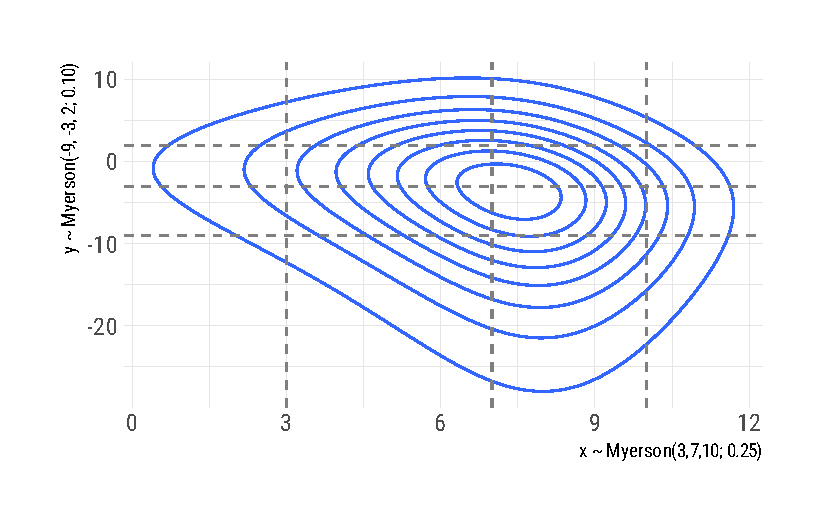
\includegraphics[width=0.8\textwidth,height=\textheight]{qpppp_files/figure-pdf/fig-bi-logitmyerson-1.pdf}

}

\caption{\label{fig-bi-logitmyerson}Density of Generalized Myerson
distributions joined by Type II bivariate logistic distribution}

\end{figure}%

Figure~\ref{fig-bi-logitmyerson} presents the Bivariate Logit-Myerson
Distribution, parameterized by \(\Theta=\{\theta_1, \theta_2, \rho\}\),
where the marginal Myerson distributions are given by
\(y_{ij}=Q_j(z(u_{ij}),\theta_j)\) for \(j=1,2\), with parameter vectors
\(\theta_1=\{3,7,10;0.25\}\), \(\theta_2=\{1,10,20;0.1\}\), and the
dependence parameter \(\beta=0.6\).

\subsection{Copula-based MQPDs}\label{copula-based-mqpds}

The approach we have used so far is similar to constructing the joint
distribution using the Gaussian copula (Hoff 2007). Copulas provide a
general approach to modeling joint distributions, separating the
bivariate dependence from the effects of marginal distributions
(Kurowicka and Cooke 2006). The literature describes a wide range of
copulas (Genest and Favre 2007; Smith 2013; Kurowicka and Joe 2011), and
new copulas can be created using generator functions (Durrleman,
Nikeghbali, and Roncalli 2000). When a copula is used to connect QPDs,
the joint density is calculated as follows:

\[
f_{MQPD}(y_1,y_2\vert \theta_1,\theta_2,\Xi)=c(F(y_1\vert\theta_1),F(y_2\vert\theta_2)\vert\Xi)
f_1\left(y_1\vert\theta_1\right) f_2\left(y_2\vert\theta_2\right)
\]

where \(c\) represents the copula density function with parameter
\(\Xi\), and \(F(y_i\vert\theta_i)\) and \(f_i(y_i\vert\theta_i)\) are
the CDF and PDF of the marginal quantile-parameterized distributions,
respectively.

The same density can be expressed in quantile-based form (Perepolkin,
Goodrich, and Sahlin 2023):

\[
[q_{MQPD}(u_1,u_2\vert\theta, \Xi)]^{-1}=c\left(u_1,u_2\vert\Xi\right)[q_1(u_1\vert\theta_1)]^{-1}[q_2(u_2\vert\theta)]^{-1}
\]

where \(c\) is the copula density function with parameter \(\Xi\), and
\([q_i(u_i\vert\theta_i)]^{-1}\), for \(i=1,2\), are the marginal DQFs
of QPDs. Figure~\ref{fig-bc-myerson} presents 10,000 samples from the
bivariate Myerson distribution joined by the Joe copula with
\(\theta=3\).

Elicitation of multivariate distributions may require a specialized
approach (Elfadaly and Garthwaite 2017; Kevin J. Wilson et al. 2021).
For examples of expert-specified multivariate distributions encoded with
copulas, we refer to (Kevin James Wilson 2018; Holzhauer et al. 2022;
Sharma and Das 2018; Aas et al. 2009). When fitting copulas to empirical
observations, the ``blanket'' goodness of fit measure (Wang and Wells
2000) based on Kendall's transform (Genest, Quessy, and Rémillard 2006;
Genest, Rémillard, and Beaudoin 2009) can be used.

\begin{figure}

\centering{

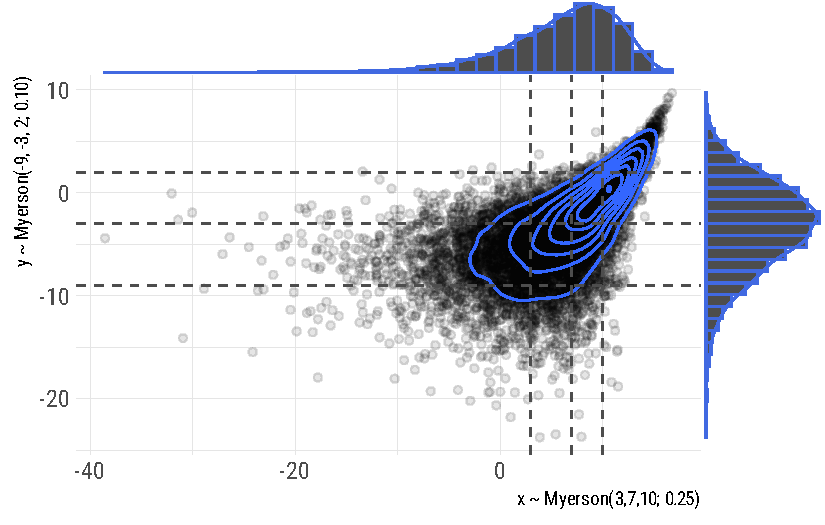
\includegraphics[width=0.8\textwidth,height=\textheight]{qpppp_files/figure-pdf/fig-bc-myerson-1.pdf}

}

\caption{\label{fig-bc-myerson}Samples from the bivariate Myerson
distribution joined by the Joe copula (\(\theta=3\))}

\end{figure}%

\subsection{Bivariate quantiles}\label{bivariate-quantiles}

The formal definition of bivariate quantile functions and the method for
constructing bivariate quantile distributions using marginal and
conditional quantile functions are provided by (Nair and Vineshkumar
2023; Vineshkumar and Nair 2019). They define the bivarate quantile
function (bQF) of \((X_1, X_2)\) as the pair
\(Q(u_1, u_2)=(Q_1(u_1), Q_{21}(u_2\vert u_1))\), where
\(Q_1(u_1)=\inf \{x_1: F_1(x_1)\geq u_1\}\), \(u_1\in[0,1]\) and
\(Q_{21}(u_2\vert u_1)=\inf\{x_2: F_{21}(Q_1, x_2)\geq u_2\}\).

The conditional quantile function \(Q_{21}(u_2\vert u_1)\) can be
obtained by inverting the conditional distribution function
\(F_{21}(x_1, x_2)\), which is computed from the factorization of the
joint survival function. The joint survival function is defined as
\(\bar{F}(x_1, x_2)=P(X_1> x_1)P(X_2> x_2 \vert X_1 > x_1)= \bar{F}(x_1)\bar{F}_{21}(x_1,x_2)\).
Note that the joint survival function
\(\bar{F}(x_1,x_2)=1-F_1(x_1)-F_2(x_2)+F(x_1,x_2)\), and the conditional
survival function \(\bar{F}_{21}(x_1,x_2)=1-F_{21}(x_1,x_2)\).

Another approach for creating bivariate quantile functions is through
Gilchrist's QF transformation rules (Gilchrist 2000), which can be
generalized to bivariate quantile functions. According to (Nair and
Vineshkumar 2023) (Property 6), the conditional QF can be constructed as
a sum of two univariate QFs:
\(Q_{21}(u_2\vert u_1) = Q_1(u_1) + Q_2(u_2)\). This means that the pair
\((Q_1(u_1), ; Q_1(u_1) + Q_2(u_2))\) is a valid bivariate quantile
function, which generalizes Gilchrist's \emph{addition rule}
(Table~\ref{tbl-qf-trans}). The addition rule also works for quantile
density functions (Property 7). If \(Q_1\) is left-bounded at zero,
i.e., \(Q_1(0) = 0\), then the margins of such a bQF are
\(X_1 = Q_1(u_1)\) and \(X_2 = Q_2(u_2)\). Otherwise, the marginal
distribution of \(X_2\) will be
\(\lim_{u_1 \rightarrow 0}Q_{21}(u_2\vert u_1)\), which in many cases is
not tractable.

If \(Q_1(u_1)\) and \(Q_2(u_2)\) are positive on \(u_i \in [0,1]\), then
their product is also a valid conditional QF (Property 8), generalizing
Gilchrist's ``product rule''. Finally, Property 9 generalizes the
``Q-transformation rule,'' stating that for every increasing
transformation functions \(T_1\) and \(T_2\),
\(\left(T_1(Q_1(u_1)), T_1(Q_1(u_1)) + T_2(Q_2(u_2))\right)\) is also a
valid bQF.

Therefore, valid bivariate quantile-parameterized QFs can be created by
constructing the conditional quantile functions as Gilchrist
combinations of univariate quantile-parameterized QFs.
Figure~\ref{fig-bq-myerson} shows 1000 samples from the bivariate
distribution created by adding together two Myerson distributions. Note
that in this case, only the marginal distribution of \(x_1 = Q_1(u_1)\)
is available in closed form.

\[
\begin{aligned}
(u_1, u_2) &\overset{X_1, X_2}{\backsim} (Q_1(u_1), Q_1(u_1)+Q_2(u_2))\\
Q_1(u_1) &\sim\text{Myerson}(3,7,10; 0.1)\\
Q_2(u_2) &\sim \text{Myerson}(-9, -3, 2; 0.25)\\
\end{aligned}
\]

This bQF is easy to elicit and interpret, since \(Q_2(u_2)\) can be
thought of as a random adjustment to the value of \(Q_1(u_1)\). In fact,
the conditional quantile function \(Q_{21}(u_2\vert u_1)\) can be
thought of as having the classical form
\(Q_{21}(u_2\vert u_1) = \mu(u_1) + \sigma Q_2(u_2)\) (Gilchrist 2000),
where the location is randomly varying with \(\mu(u_1) = Q_1(u_1)\) and
the scale parameter \(\sigma = 1\). First, the marginal distribution
\(Q_1(u_1)\) is elicited, and then the difference between the values
\(x_1\) and \(x_2\) can be elicited as a QPT and encoded as
\(Q_2(u_2)\).

\begin{figure}

\centering{

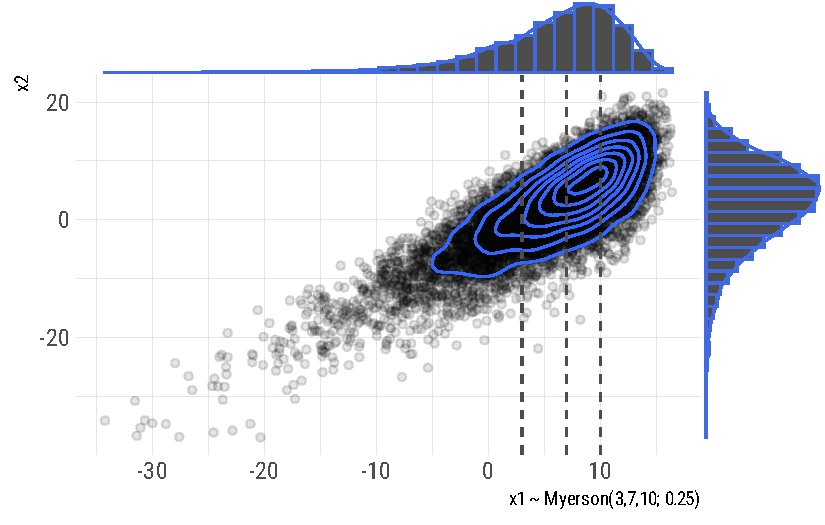
\includegraphics[width=0.8\textwidth,height=\textheight]{qpppp_files/figure-pdf/fig-bq-myerson-1.pdf}

}

\caption{\label{fig-bq-myerson}Samples from the Bivariate Myerson
quantile function}

\end{figure}%

\section{Discussion}\label{discussion}

Quantile-based distributions have garnered significant attention in the
research community. Several distributions, such as the Generalized
Lambda Distribution (GLD) (Freimer et al. 1988; Ramberg and Schmeiser
1974), the g-and-k distribution (M. A. Haynes, MacGillivray, and
Mengersen 1997; M. Haynes and Mengersen 2005; Jacob 2017; Prangle 2017),
the g-and-h distribution (Field and Genton 2006; Mac Gillivray 1992;
Rayner and MacGillivray 2002), and the Wakeby distribution (Jeong-Soo
2005; Rahman et al. 2015; Tarsitano 2005a), have been extensively
studied and documented in the literature. These distributions are
defined by non-invertible quantile functions (Perepolkin, Goodrich, and
Sahlin 2023). However, the research on quantile-parameterized
distributions remains relatively unexplored. These distributions offer
interpretable parameters that are defined on the same scale as the
quantities of interest, simplifying the elicitation process for experts.
Many popular elicitation protocols for both predictive and parametric
elicitation rely on the assessment of quantile-probability pairs (QPPs).
Instead of fitting a parametric distribution to the elicited QPPs (Best,
Dallow, and Montague 2020; O'Hagan 2019), assessors could directly use
the elicited QPPs as inputs into one of the QPD quantile functions,
which can be easily employed in both quantile-parameterized and
parametric models.

Provided that the expert and the elicitor agree on the scientific model
to be used for representing the expert's understanding of the world
(Burgman, Layman, and French 2021), several types of inputs may be
required to inform the model. Among those are the expert's judgement
about the model \emph{parameters} (Mikkola et al. 2021; O'Hagan 2019)
and their \emph{predictions} of the next observation (Akbarov 2009; J.
Kadane and Wolfson 1998; Winkler 1980). Both parametric and predictive
judgments should be captured together with corresponding uncertainties
to reflect the expert's state of knowledge. Quantile-parameterized
distributions offer distinct advantages as high-fidelity priors that
precisely capture expert assessments. These distributions are
particularly beneficial for domain experts who may not be well-versed in
statistics, as they provide high flexibility while retaining parameter
interpretability. As a result, QPDs can faithfully represent an expert's
beliefs without compromising convenience or precision.

Different quantile-parameterized distributions fitted to the same set of
quantile-probability pairs may exhibit slight variations in shape.
However, given the diverse range of QPDs proposed in the literature a
knowledgeable assessor should be able to select an appropriate
distribution and validate the choice with the expert, taking into
account the thickness of the distribution tails.

Most QPDs we reviewed are parameterized by a symmetric percentile
triplet (SPT). These distributions rely on the symmetric property of
underlying \emph{kernel} distributions and can be generalized by
swapping the distribution with another one that exhibits different tail
shapes. Hadlock and Bickel (Christopher C. Hadlock and Bickel 2019)
utilized this method to generalize Johnson Quantile Parameterized
distributions (J-QPDs). We show that the variants of Myerson
distribution appearing in the literature (Myerson 2005; Kevin J. Wilson
et al. 2023) represent similar generalization. This principle can be
extended to include other kernels which result in varying thickness of
the tails.

\subsubsection*{Quantile function
perspective}\label{quantile-function-perspective}
\addcontentsline{toc}{subsubsection}{Quantile function perspective}

The distributions discussed in this paper are defined using the quantile
function and, therefore, they can be considered \emph{quantile-based}
quantile-parameterized distributions. Myerson, J-QPD, and several other
quantile-parameterized distributions reparameterize conventional
distributions, utilizing Gilchrist's Quantile Function (QF)
transformations (Gilchrist 2000).

Perepolkin et al. (Perepolkin, Goodrich, and Sahlin 2023) demonstrated
that the distributions defined by the quantile function can be used both
as prior and as likelihood in Bayesian models. Priors defined by the
quantile function eliminate the need to compute prior density. The
quantile function acts as a non-linear transformation of a uniform
degenerate random variate with the resulting Jacobian adjustment
reciprocal to the density quantile function. Therefore, both the
Jacobian and the density quantile function are omitted from the Bayesian
updating equation (Perepolkin, Goodrich, and Sahlin 2023). When using
quantile-based QPDs as likelihood, special care needs to be taken with
regards to the suitable prior for the QPP parameters. (Perepolkin,
Goodrich, and Sahlin 2021) used the Dirichet-based prior for the metalog
likelihood model and descibed the \emph{hybrid} elicitation process for
encoding the expert judgments into the two-dimensional prior
distribution implied by the model.

\subsubsection*{Feasibility of
parameters}\label{feasibility-of-parameters}
\addcontentsline{toc}{subsubsection}{Feasibility of parameters}

Not all QPDs are equally reliable in approximating the underlying
distributions. Violating the QF transformation rules imposes additional
constraints on the feasibility of parameters, as certain combinations of
parameters may result in locally decreasing quantile functions (Keelin
2016; Christopher Campbell Hadlock 2017). We discussed this limitation
in relation to SQN and metalog distributions, but the same challenges
affect other distributions with QF violating Gilchrist QF transformation
rules. In this regard, the quantile-parameterized model, which relies on
Gilchrist combination of basic quantile functions, proposed by (Peng,
Li, and Uryasev 2023), represents a highly promising advancement.
Weighted constrained optimization algorithm ensuring that the quantile
mixture weights remain non-negative opens new possibilities for other
QPDs using monotonic transformations of quantile functions. The
estimator proposed by (Peng, Li, and Uryasev 2023) is asymptotically a
q-Wasserstein distance, which has also been used for parameter
estimation in Approximate Bayesian Computation (Bernton et al. 2019).

The feasibility conditions for the Generalized Lambda Distribution (GLD)
have been a focal point of numerous research endeavors in the past (Dean
2013; Fournier et al. 2007; Karian and Dudewicz 2019; King and
MacGillivray 2007; Tarsitano 2005b, etc). Various reparameterizations
have been explored to enhance parameter identifiability (Ramberg and
Schmeiser 1974). Recently, (Chalabi, Scott, and Wuertz 2012) proposed a
novel asymmetry-skewness reparameterization for the previously popular
Freimer, Kollia, Mudholkar \& Lin version of GLD (FKML GLD) (Freimer et
al. 1988), wherein two of the four parameters are mapped to robust
quantile-based moments, namely the median and Interquartile Range (IQR).
This reduction in the number of parameters required for data fitting
simplifies the previously computationally intensive fitting algorithms.
As demonstrated in the plot of robust moments
(Figure~\ref{fig-unbounded}) GLD remains one of the most flexible
unbounded distributions, capable of accommodating a wide range of
shapes. (Dedduwakumara, Prendergast, and Staudte 2021) described a
two-step method for fitting FKML GLD using the probability density
quantile function (Staudte 2017). However, when applying their method to
fitting the CSW GLD, the second step becomes unnecessary as the location
and scale can be directly mapped to the empirical first and second
robust moments.

CSW GLD represents a prime example of clever reparameterization aiming
at alleviating the deficiencies of QF construction through setting
consistent parameter boundaries and defining fall-back cases for an
impossible combination of parameters. This degree of reparameterization
is difficult for QPDs because the objective is to retain the mapping of
parameters to the valid set of quantile-probability pairs. Therefore,
for improperly constructed QPDs the feasibility conditions will have to
be expressed as ratios of quantiles.

\subsubsection*{Multivariate extensions}\label{multivariate-extensions}
\addcontentsline{toc}{subsubsection}{Multivariate extensions}

Quantile-parameterized distributions can be readily extended to the
multivariate setting by leveraging traditional multivariate
distributions. The combination of quantile-based marginal distributions
joined by the multivariate normal has been previously discussed in the
literature (Drovandi and Pettitt 2011; Hoff 2007). Building on this
approach, we proposed the use of Gumbel's bivariate logistic
distribution (Gumbel 1961) to combine quantile-parameterized
Logit-Myerson distributions (Kevin J. Wilson et al. 2023).

Copulas offer a natural extension of univariate QPDs into the
multivariate domain. Bivariate copulas can be assembled into more
complex structures using vine copulas (Czado 2019; Kurowicka and Joe
2011; Kevin James Wilson 2018). Flexible QPDs serve as a viable
alternative to empirical copulas, where the margins are represented by
kernel density estimation (KDE) or other non-parametric approaches.
Poorly fitted marginal distributions mean \emph{less-than-ideal}
starting point for copula modeling, because of deviations from
uniformality of the copula margins.

Quantile-parameterized distributions defined by the quantile function
are particularly well-suited for constructing new distributions using
bivariate quantiles (Nair and Vineshkumar 2023; Vineshkumar and Nair
2019). The ability to construct a conditional quantile function as a
Gilchrist combination of univariate quantile functions offers a
convenient and interpretable approach to defining bivariate
distributions, especially when the univariate quantile functions are
parameterized by quantiles. These distributions are easy to sample from
and construct. However, fitting these distributions to data or posterior
samples can be challenging. As shown by (Castillo, Sarabia, and Hadi
1997) the fitting process requires all marginal and conditional quantile
functions to be available in closed form, which is often unattainable.

\subsubsection*{Further research}\label{further-research}
\addcontentsline{toc}{subsubsection}{Further research}

There appears to be a limited availability of unbounded
quantile-parameterized distributions in the current literature. Among
the distributions we examined, only the metalog distribution and
quantile mixtures can extend across the entire real line. The G-QPD
system provides clear distributional bounds explicitly defined by the
expert during elicitation. In contrast, the (Generalized) Myerson
distribution system relies on implicit bounds that need to be
communicated to the expert. Most of the distributions we reviewed are
characterized by a symmetrical percentile triplet (SPT), as they rely on
the symmetrical property of their kernels. However, there may be
situations where an arbitrary (non-symmetrical) quantile
parameterization could prove valuable (as shown by Perepolkin, Goodrich,
and Sahlin 2021). The development of flexible quantile-parameterized
distributions defined by an arbitrary set of quantile-probability pairs
using quantile mixtures (Peng, Li, and Uryasev 2023) can enhance
versatility of QPDs and facilitate their broader adoption.

In conclusion, quantile-parameterized distributions offer a valuable
framework for capturing expert assessments and incorporating them into
statistical models. They provide high flexibility and parameter
interpretability, making them particularly beneficial for domain
experts. The diverse range of quantile-parameterized distributions
explored in the literature allows for customized modeling approaches
that align with the expert's beliefs and uncertainties. By embracing
these innovative distributions, researchers and practitioners can
enhance the accuracy and reliability of their statistical models while
leveraging expert knowledge effectively.

\section*{Miscellaneous}\label{miscellaneous}
\addcontentsline{toc}{section}{Miscellaneous}

\subsection*{Acknowledgments}\label{acknowledgments}
\addcontentsline{toc}{subsection}{Acknowledgments}

The authors have no conflict of interest to declare. U Sahlin was funded
by the Crafoord Foundation (ref 20200626). We thank the editorial team
and reviewers for their constructive feedback which helped us improve
this manuscript.

\subsection*{ORCID}\label{orcid}
\addcontentsline{toc}{subsection}{ORCID}

Dmytro Perepolkin https://orcid.org/0000-0001-8558-6183\\
Erik Lindström https://orcid.org/0000-0002-6468-2624\\
Ullrika Sahlin http://orcid.org/0000-0002-2932-6253

\section*{Appendix A. Distribution
functions}\label{appendix-a.-distribution-functions}
\addcontentsline{toc}{section}{Appendix A. Distribution functions}

\subsection*{Myerson Distribution}\label{myerson-distribution-1}
\addcontentsline{toc}{subsection}{Myerson Distribution}

The derivative of the quantile function with respect to the depth \(u\)
is the Quantile Density Function, which for Myerson distribution has the
following form

\[
q(u\vert q_1,q_2,q_3,\alpha)=\begin{cases}
\rho\frac{\beta^\kappa\ln(\beta)}{(\beta-1)}\frac{q_{norm}(u)}{\Phi^{-1}(1-\alpha)}, \quad &\beta \neq 1\\
\rho\frac{q_{norm}(u)}{\Phi^{-1}(1-\alpha)}, \quad &\beta = 1
\end{cases}
\]

where \(q_{norm}=\frac{d\Phi^{-1}(u)}{du}\) is the quantile density
function for the standard normal distribution.

The Myerson distribution is invertible. The distribution function of
random variable \(X\) has the form

\[
\begin{aligned}\;
\psi&=\Phi^{-1}(1-\alpha)\left(\frac{\ln\left(1+\frac{(x-q_2)(\beta-1)}{\rho}\right)}{\ln(\beta)}\right)&\\
F(x\vert q_1, q_2, q_3, \alpha)&=\begin{cases}
\Phi(\psi), \quad &\beta\neq 1\\
F_{normal}(x\vert q_2,\rho/\Phi^{-1}(1-\alpha) ), \quad &\beta=1
\end{cases}
\end{aligned}
\]

where \(\Phi()\) is the CDF of the standard normal distribution and
\(\Phi^{-1}()\) is its inverse.
\(F_{normal}(x\vert q_2,\rho/\Phi^{-1}(1-\alpha))\) is the CDF of the
normal distribution with mean \(\mu=q_2\) and standard deviation
\(\sigma=\rho/\Phi^{-1}(1-\alpha)\).

The derivative of the distribution function with respect to the random
variable \(X\) is the probability density function, which for the
Myerson distribution takes the following form

\[
f(x\vert q_1, q_2, q_3, \alpha)=\begin{cases}
\frac{\Phi^{-1}(1-\alpha)(\beta-1)}{(\rho+(x-q_2)(\beta-1))\ln(\beta)}\varphi(\psi), \quad &\beta\neq1\\
f_{normal}(x\vert q_2,\rho/\Phi^{-1}(1-\alpha)),\quad &\beta=1
\end{cases}
\]

where \(\varphi()\) is the probability density function of the standard
normal distribution,
\(f_{normal}(x\vert q_2,\frac{\rho}{\Phi^{-1}(1-\alpha)})\) is the PDF
of the normal distribution with the mean \(\mu=q_2\) and standard
deviation \(\sigma=\rho/\Phi^{-1}(1-\alpha))\).

\subsection*{Generalized Myerson
Distributions}\label{generalized-myerson-distributions}
\addcontentsline{toc}{subsection}{Generalized Myerson Distributions}

The Quantile Density Function of Generalized Myerson Distribution for
\(u\neq0, u\neq1\) is

\[
q_M(u\vert q_1,q_2,q_3,\alpha)=\begin{cases}
\rho\frac{\beta^\kappa\ln(\beta)}{(\beta-1)}\frac{s(u)}{S(1-\alpha)}, \quad &\beta \neq 1\\
\rho\frac{s(u)}{S(1-\alpha)}, \quad &\beta = 1
\end{cases}
\]

where \(S(u)\) is the quantile function and \(s(u)=\frac{dS(u)}{du}\) is
the quantile density function for the kernel distribution. When \(u=0\)
or \(u=1\) the \(q_M(u)=\infty\).

The Generalized Myerson distribution is invertible. The distribution
function of random variable \(X\) has the form

\[
\begin{aligned}\;
\psi &=S(1-\alpha)\left(\frac{\ln\left(1+\frac{(x-q_2)(\beta-1)}{\rho}\right)}{\ln(\beta)}\right)\\
F_M(x\vert q_1, q_2, q_3, \alpha)&=\begin{cases}
F(\psi), \quad &\beta\neq 1\\
q_2+ \frac{\rho}{S(1-\alpha)}F(x), \quad &\beta=1
\end{cases}
\end{aligned}
\]

where \(F()\) is the standard CDF of the kenel distribution and \(S()\)
is its inverse.

The derivative of the distribution function with respect to the random
variable \(X\) is the probability density function, which for the
Myerson distribution takes the following form

\[
f_M(x\vert q_1, q_2, q_3, \alpha)=\begin{cases}
\frac{S(1-\alpha)(\beta-1)}{(\rho+(x-q_2)(\beta-1))\ln(\beta)}f(\psi), \quad &\beta\neq1\\
f\left(\frac{x-q_2}{\rho/S(1-\alpha)}\right),\quad &\beta=1
\end{cases}
\]

where \(f()\) is the probability density function of the standard kernel
distribution. Compare it to the simplicity of the Quantile Density
Function above.

\subsection*{Johnson Quantile-Parameterized
Distribution}\label{johnson-quantile-parameterized-distribution-1}
\addcontentsline{toc}{subsection}{Johnson Quantile-Parameterized
Distribution}

The JQPD-B quantile density function can be computed as

\[
q_B(p)=\begin{cases}
(u_b-l_b)\varphi(\xi+\lambda\sinh(\delta(z(p)+nc))) \times\\
\quad \lambda\cosh(\sigma(z(p)+nc)) \sigma q_{norm}(p), \quad &n\neq 0\\
(u_b-l_b)\varphi\left(B+\left(\frac{H-L}{2c}\right)z(p)\right)
\times \left(\frac{H-L}{2c}\right)q_{norm}(p), \quad &n=0
\end{cases}
\]

The JQPD-B distribution function

\[
F_B(x)=\begin{cases}
\Phi\left((2c/(H-L))(-B+z\left(\frac{x-l}{u-l}\right))\right), \quad &n=0 \\
\Phi\left(\frac{1}{\delta}\sinh^{-1}\left(\frac{1}{\lambda}\left(z\left(\frac{x-l}{u-l}\right)-\xi\right)\right)-nc\right), \quad &n\neq0
\end{cases}
\]

The JQPD-B probability density function (PDF) is

\[
\begin{gathered}
f(x)=\begin{cases}
\frac{2c}{(H-L)(u_b-l_b)}\frac{1}{\varphi\left(z\left(\frac{x-l_b}{u_b-l_b}\right)\right)}\varphi\left(\frac{2c}{H-L}\left(-B+z\left(\frac{x-l_b}{u-l_b}\right)\right)\right), \quad &n=0\\
\frac{1}{\delta}\frac{1}{u_b-l_b}\varphi\left(-nc+\frac{1}{\delta}\sinh^{-1}\left(\frac{1}{\lambda}\left(-\xi+z\left(\frac{x-l_b}{u_b-l_b}\right)\right)\right)\right) \times \\ \indent
\frac{1}{\varphi\left(z\left(\frac{x-l_b}{u_b-l_b}\right)\right)}\frac{1}{\sqrt{\lambda^2+\left(-\xi+z\left(\frac{x-l_b}{u_b-l_b}\right)\right)^2}}, \quad &n\neq 0\\
\end{cases}
\end{gathered}
\]

J-QPD-S quantile density function

\[
q_S(p)=\begin{cases}
\theta\exp\left(\lambda\delta z(p)\right)\lambda\delta q_{norm}(p), \quad &n=0\\
\theta\exp\left(\lambda\sinh^{-1}(\delta z(p))+\sinh^{-1}(nc\delta)\right)\lambda\frac{1}{\sqrt{1+(\delta z(p))^2}}\delta q_{norm}(p), \quad &n\neq0\\
\end{cases}
\]

J-QPD-S distribution function

\[
F_S(x)=\begin{cases}
F_{lnorm}(x-l_b\vert \ln(\theta), \frac{H-B}{c}), \quad &n=0\\
\Phi\left(\frac{1}{\delta}\sinh\left(\sinh^{-1}\left(\frac{1}{\lambda}\ln\frac{x-l_b}{\theta}\right)-\sinh^{-1}(nc\delta)\right)\right), \quad &n\neq0\\
\end{cases}
\]

J-QPD-S probability density function (PDF)

\[
f_S(x)=\begin{cases}
\frac{1}{x\sigma\sqrt{2\pi}}\exp\left(-\frac{(\ln x-ln\xi)^2}{2\frac{(H-B)^2}{c^2}}\right), \quad &n=0\\
\varphi\left(\frac{\sinh(\sinh^{-1}(cn\sigma)-\sinh^{-1}(\frac{1}{\lambda}\ln\frac{x-l_b}{\theta}))}{\delta}\right)\frac{\cosh(\sinh^{-1}(cn\delta)-\sinh^{-1}(\frac{1}{\lambda}\ln\frac{x-l_b}{\theta}))}{(x-l_b)\delta\lambda\sqrt{1+\left(\frac{\ln\frac{x-l_b}{\theta}}{\lambda}\right)^2}}, \quad &n \neq 0
\end{cases}
\]

where \(\mu=\ln\xi\) and \(\sigma=\frac{H-B}{c}\).

\subsection*{Metalog distribution}\label{metalog-distribution}
\addcontentsline{toc}{subsection}{Metalog distribution}

This section recapitulates ideas and formulas provided in (Keelin 2016)
with our own notation and minor reinterpretations.

Metalog distribution is created from the logistic quantile function
\(Q(p)=\mu+s\text{logit}(p)\), where \(\mu\) is the mean, \(s\) is
proportional to the standard deviation such that \(\sigma=s\pi/\sqrt3\),
\(p\) is the probability \(p \in [0,1]\). The metalog quantile function
is built by substitution and series expansion of its parameters \(\mu\)
and \(s\) with the polynomial of the form:

\[
\begin{aligned}\;
&\mu=a_1+a_4(p-0.5)+a_5(p-0.5)^2+a_7(p-0.5)^3+a_9(p-0.5)^4+\dots, \\
& s=a_2+a_3(p-0.5)+a_6(p-0.5)^2+a_8(p-0.5)^3+a_{10}(p-0.5)^4+\dots,
\end{aligned}
\]

where \(a_i, \; i \in (1\dots n)\) are real constants. Given a
size-\(m\) QPT \(\{p, q\}_m\), where \(p=\{p_1\dots p_m\}\) and
\(q=\{q_1\dots q_m\}\) the vector of coefficients \(a=\{a_1\dots a_m\}\)
can be determined through the set of linear equations.

\[
\begin{aligned}\;
&q_1=a_1+a_2\text{logit}(p_1)+a_3(p_1-0.5)\text{logit}(p_1)+a_4(p_1-0.5)+\cdots,\\
&q_2=a_1+a_2\text{logit}(p_2)+a_3(p_2-0.5)\text{logit}(p_2)+a_4(p_2-0.5)+\cdots,\\
&\vdots\\
&q_m=a_1+a_2\text{logit}(p_m)+a_3(p_m-0.5)\text{logit}(p_m)+a_4(p_m-0.5)+\cdots.\\
\end{aligned}
\]

In the matrix form, this system of equations is equivalent to
\(q=\mathbb{P}a\), where \(q\) and \(a\) are column vectors and
\(\mathbb{P}\) is a \(m \times n\) matrix:

\[
\mathbb{P} = \left[\begin{array}{lllll}
1  &\text{logit}(p_1) &(p_1-0.5)\text{logit}(p_1) &(p_1-0.5) &\cdots\\
1  &\text{logit}(p_2) &(p_2-0.5)\text{logit}(p_2) &(p_2-0.5) &\cdots\\
   &                  &\vdots\\
1  &\text{logit}(p_m) &(p_m-0.5)\text{logit}(p_m) &(p_m-0.5) &\cdots
\end{array}\right]
\]

If \(m=n\) and \(\mathbb{P}\) is invertible, then the vector of
coefficients \(a\) of this \emph{properly parameterized} metalog QPD can
be uniquely determined by

\begin{equation}\phantomsection\label{eq-nmetalogAsMatrixeq}{
a=\mathbb{P}^{-1}q
}\end{equation}

If \(m > n\) and \(\mathbb{P}\) has a rank of at least \(n\), then the
vector of coefficients \(a\) of the \emph{approximated} metalog QPD, can
be estimated using

\[
a=[\mathbb{P}^T\mathbb{P}]^{-1}\mathbb{P}^Tq
\]

The matrix to be inverted is always \(n \times n\) regardless of the
size \(m\) of QPT used.

Metalog \emph{quantile function} (QF) with \(n\) terms
\(Q_{M_n}(u\vert a)\) can be expressed as

\begin{equation}\phantomsection\label{eq-metalogQFeq}{
Q_{M_n}(u\vert a)=\begin{cases}
a_1+a_2\text{logit}(u), \text{ for } n=2, \\
a_1+a_2\text{logit}(u)+a_3(u-0.5)\text{logit}(u), \text{ for } n=3, \\
a_1+a_2\text{logit}(u)+a_3(u-0.5)\text{logit}(u)+a_4(u-0.5), \text{ for } n=4, \\
Q_{M_{n-1}} + a_n(u-0.5)^{(n-1)/2}, \text{ for odd } n \geq 5, \\
Q_{M_{n-1}} + a_n(u-0.5)^{n/2-1}\text{logit}(u), \text{ for even } n \geq 6, \\
\end{cases}
}\end{equation}

where \(u \in [0,1]\) is the cumulative probability and \(a\) is the
size-\(n\) parameter vector of real constants \(a=\{a_1\dots a_n\}\).

The metalog \emph{quantile density function} (QDF) can be found by
differentiating the Equation~\ref{eq-metalogQFeq} with respect to \(u\):

\begin{equation}\phantomsection\label{eq-metalogQDFeq}{
\begin{gathered}
q_{M_n}(u\vert a)=\begin{cases}
a_2\mathcal I(u), \text{ for } n=2, \\
a_2\mathcal I(u)+a_3\left((u-0.5)\mathcal I(u)+\text{logit}(u) \right), \text{ for } n=3, \\
a_2\mathcal I(u) + a_3\left((u-0.5)\mathcal I(u)+\text{logit}(u) \right)+ a_4,  \text{ for } n=4, \\
q_{M_{n-1}} + 0.5a_n(n-1)(u-0.5)^{(n-3)/2}, \text{ for odd } n \geq 5, \\
q_{M_{n-1}} + a_n((u-0.5)^{n/2-1}\mathcal I(u)+\\ \indent (0.5n-1)(u-0.5)^{n/2-2}\text{logit}(u)), \text{ for even } n \geq 6, \\
\end{cases}
\end{gathered}
}\end{equation}

where \(\mathcal I(u)=[u(1-u)]^{-1}\). The constants \(a\) are feasible
iif \(q_{M_{n}}(u\vert a)>0, \;\forall u \in [0,1]\).

Metalog \emph{density quantile function} (DQF), referred to as the
``metalog pdf'' in (Keelin 2016) can be obtained by
\(f(Q_{M_n}(u\vert a))=[q_{M_n}(u\vert a)]^{-1}\).

Metalog \emph{cumulative distribution function} (CDF)
\(F_{M_n}(x\vert a)\) does not have an explicit form because
\(Q_{M_n}(u\vert a)\) is not invertible (Keelin 2016). It is, however,
possible to approximate \(\widehat Q^{-1}_{M_n}(x\vert a)\) using
approximation.

Metalog distribution is defined for all \(x \in \mathbb R\) on the real
line. (Keelin 2016) provides semi-bounded \emph{log-metalog}, and the
bounded \emph{logit-metalog} variations of the metalog distribution. As
the names suggest, this is achieved through the variable substitution
with \(z=\ln(x-b_l)\) or \(z=-\ln(b_u-x)\) for the semi-bounded case,
and \(z=\ln((x-b_l)/(b_u-x))\) for the bounded case, where \(z\) is
metalog-distributed and \(b_l, b_u\) are the lower and upper limits,
respectively. Substituting one of the transformations into the QF and
QDF functions above, yields semi-bounded or bounded metalog
distribution. For the exact formulae of the log-metalog and
logit-metalog refer to (Keelin 2016).

\subsection*{CSW GLD}\label{csw-gld}
\addcontentsline{toc}{subsection}{CSW GLD}

Quantile density function for the CSW GLD is provided in (Chalabi,
Scott, and Wuertz 2012)

\[
\begin{gathered}
q(u\vert\tilde\sigma,\chi,\xi)= \frac{\tilde\sigma}{S(0.75\vert\chi,\xi)-S(0.25\vert\chi,\xi)}
s(u\vert\chi,\xi) \\
s(u\vert\chi,\xi)=\frac{d}{du}S(u\vert\chi,\xi)=u^{\alpha+\beta-1}+(1-u)^{\alpha-\beta-1}
\end{gathered}
\]

\newpage{}

\section*{References}\label{references}
\addcontentsline{toc}{section}{References}

\phantomsection\label{refs}
\begin{CSLReferences}{1}{0}
\bibitem[\citeproctext]{ref-aas2009PaircopulaConstructionsMultiple}
Aas, Kjersti, Claudia Czado, Arnoldo Frigessi, and Henrik Bakken. 2009.
{``Pair-Copula Constructions of Multiple Dependence.''} \emph{Insurance:
Mathematics and Economics} 44 (2): 182--98.
\url{https://doi.org/bmnchh}.

\bibitem[\citeproctext]{ref-akbarov2009ProbabilityElicitationPredictive}
Akbarov, A. 2009. {``Probability Elicitation: {Predictive} Approach.''}
PhD thesis, University of Salford.

\bibitem[\citeproctext]{ref-arachchige2022RobustAnalogsCoefficient}
Arachchige, Chandima N. P. G., Luke A. Prendergast, and Robert G.
Staudte. 2022. {``Robust Analogs to the Coefficient of Variation.''}
\emph{Journal of Applied Statistics} 49 (2): 268--90.
\url{https://doi.org/10.1080/02664763.2020.1808599}.

\bibitem[\citeproctext]{ref-basikhasteh2021BayesianEstimationMorgenstern}
Basikhasteh, Mehdi, Fazlollah Lak, and Saeid Tahmasebi. 2021.
{``Bayesian {Estimation} of {Morgenstern Type Bivariate Rayleigh
Distribution Using Some Types} of {Ranked Set Sampling}.''}
\emph{Revista Colombiana de Estad{í}stica} 44 (2): 279--96.
\url{https://doi.org/10.15446/rce.v44n2.87825}.

\bibitem[\citeproctext]{ref-berkson1951WhyPreferLogits}
Berkson, Joseph. 1951. {``Why {I Prefer Logits} to {Probits}.''}
\emph{Biometrics} 7 (4): 327--39. \url{https://doi.org/10.2307/3001655}.

\bibitem[\citeproctext]{ref-bernton2019ParameterEstimationWasserstein}
Bernton, Espen, Pierre E Jacob, Mathieu Gerber, and Christian P Robert.
2019. {``On Parameter Estimation with the {Wasserstein} Distance.''}
\emph{Information and Inference: A Journal of the IMA} 8 (4): 657--76.
\url{https://doi.org/10.1093/imaiai/iaz003}.

\bibitem[\citeproctext]{ref-best2020PriorElicitation}
Best, Nicky, Nigel Dallow, and Timothy Montague. 2020. {``Prior
Elicitation.''} \emph{Bayesian Methods in Pharmaceutical Research},
87--109. \url{https://doi.org/10.1201/9781315180212-5}.

\bibitem[\citeproctext]{ref-boos1986BootstrapMethodsUsing}
Boos, Dennis D., and John F. Monahan. 1986. {``Bootstrap {Methods Using
Prior Information}.''} \emph{Biometrika} 73 (1): 77--83.
\url{https://doi.org/10.2307/2336273}.

\bibitem[\citeproctext]{ref-bowley1920ElementsStatistics}
Bowley, Arthur Lyon. 1920. \emph{Elements of Statistics}. New York, NY:
Scribner's.

\bibitem[\citeproctext]{ref-brand2019CumulativeScienceBayesian}
Brand, Charlotte Olivia, James Patrick Ounsley, Daniel Job van der Post,
and Thomas Joshua Henry Morgan. 2019. {``Cumulative {Science} via
{Bayesian Posterior Passing}: {An Introduction}.''}
\emph{Meta-Psychology} 3 (June).
\url{https://doi.org/10.15626/MP.2017.840}.

\bibitem[\citeproctext]{ref-burgman2021ElicitingModelStructures}
Burgman, Mark, Hannah Layman, and Simon French. 2021. {``Eliciting
{Model Structures} for {Multivariate Probabilistic Risk Analysis}.''}
\emph{Frontiers in Applied Mathematics and Statistics} 7.
\url{https://doi.org/10.3389/fams.2021.668037}.

\bibitem[\citeproctext]{ref-castillo1997FittingContinuousBivariate}
Castillo, Enrique, José María Sarabia, and Ali S. Hadi. 1997. {``Fitting
Continuous Bivariate Distributions to Data.''} \emph{Journal of the
Royal Statistical Society: Series D (The Statistician)} 46 (3): 355--69.
\url{https://doi.org/10.1111/1467-9884.00089}.

\bibitem[\citeproctext]{ref-chalabi2012FlexibleDistributionModeling}
Chalabi, Yohan, David J Scott, and Diethelm Wuertz. 2012. {``Flexible
Distribution Modeling with the Generalized Lambda Distribution.''}
Working Paper MPRA Paper No. 43333,. Zurich, Switzerland: ETH.

\bibitem[\citeproctext]{ref-cullen1999ProbabilisticTechniquesExposure}
Cullen, Alison C, H Christopher Frey, and Christopher H Frey. 1999.
\emph{Probabilistic Techniques in Exposure Assessment: A Handbook for
Dealing with Variability and Uncertainty in Models and Inputs}. Springer
Science \& Business Media.

\bibitem[\citeproctext]{ref-czado2019AnalyzingDependentData}
Czado, Claudia. 2019. \emph{Analyzing Dependent Data with Vine Copulas}.
New York, NY: Springer Berlin Heidelberg.

\bibitem[\citeproctext]{ref-dean2013ImprovedEstimationRegression}
Dean, Benjamin. 2013. {``Improved Estimation and Regression Techniques
with the Generalised Lambda Distribution.''} PhD thesis, Callaghan,
Australia: University of Newcastle.

\bibitem[\citeproctext]{ref-dedduwakumara2021EfficientEstimatorParameters}
Dedduwakumara, Dilanka S., Luke A. Prendergast, and Robert G. Staudte.
2021. {``An Efficient Estimator of the Parameters of the Generalized
Lambda Distribution.''} \emph{Journal of Statistical Computation and
Simulation} 91 (1): 197--215.
\url{https://doi.org/10.1080/00949655.2020.1808979}.

\bibitem[\citeproctext]{ref-drovandi2011LikelihoodfreeBayesianEstimation}
Drovandi, Christopher C., and Anthony N. Pettitt. 2011.
{``Likelihood-Free {Bayesian} Estimation of Multivariate Quantile
Distributions.''} \emph{Computational Statistics \& Data Analysis} 55
(9): 2541--56. \url{https://doi.org/10.1016/j.csda.2011.03.019}.

\bibitem[\citeproctext]{ref-dunson2005ApproximateBayesianInference}
Dunson, David B., and Jack A. Taylor. 2005. {``Approximate {Bayesian}
Inference for Quantiles.''} \emph{Journal of Nonparametric Statistics}
17 (3): 385--400. \url{https://doi.org/10.1080/10485250500039049}.

\bibitem[\citeproctext]{ref-durrleman2000SimpleTransformationCopulas}
Durrleman, Valdo, Ashkan Nikeghbali, and Thierry Roncalli. 2000. {``A
Simple Transformation of Copulas.''} \emph{Available at SSRN 1032543}.
\url{https://doi.org/10.2139/ssrn.1032543}.

\bibitem[\citeproctext]{ref-efsa2023RiskAssessmentCitripestis}
EFSA, Panel on Plant Health, Claude Bragard, Paula Baptista, Elisavet
Chatzivassiliou, Francesco Di Serio, Paolo Gonthier, Josep Anton Jaques
Miret, et al. 2023. {``Risk Assessment of {Citripestis} Sagittiferella
for the {EU}.''} \emph{EFSA Journal} 21 (2): e07838.
\url{https://doi.org/10.2903/j.efsa.2023.7838}.

\bibitem[\citeproctext]{ref-elfadaly2017ElicitingDirichletGaussian}
Elfadaly, Fadlalla G., and Paul H. Garthwaite. 2017. {``Eliciting
{Dirichlet} and {Gaussian} Copula Prior Distributions for Multinomial
Models.''} \emph{Statistics and Computing} 27 (2): 449--67.
\url{https://doi.org/10.1007/s11222-016-9632-7}.

\bibitem[\citeproctext]{ref-field2006MultivariateGandhDistribution}
Field, Christopher, and Marc G Genton. 2006. {``The {Multivariate}
g-and-h {Distribution}.''} \emph{Technometrics} 48 (1): 104--11.
\url{https://doi.org/10.1198/004017005000000562}.

\bibitem[\citeproctext]{ref-fiori2009KarlPearsonOrigin}
Fiori, Anna M., and Michele Zenga. 2009. {``Karl {Pearson} and the
Origin of Kurtosis.''} \emph{International Statistical Review} 77 (1):
40--50. \url{https://doi.org/10.1111/j.1751-5823.2009.00076.x}.

\bibitem[\citeproctext]{ref-fournier2007EstimatingParametersGeneralized}
Fournier, Benjamin, Nicolas Rupin, Maxence Bigerelle, Denis Najjar,
Alain Iost, and R Wilcox. 2007. {``Estimating the Parameters of a
Generalized Lambda Distribution.''} \emph{Computational Statistics \&
Data Analysis} 51 (6): 2813--35.
\url{https://doi.org/10.1016/j.csda.2006.09.043}.

\bibitem[\citeproctext]{ref-freimer1988StudyGeneralizedTukey}
Freimer, Marshall, Georgia Kollia, Govind S Mudholkar, and C Thomas Lin.
1988. {``A Study of the Generalized {Tukey} Lambda Family.''}
\emph{Communications in Statistics-Theory and Methods} 17 (10):
3547--67. \url{https://doi.org/10.1080/03610928808829820}.

\bibitem[\citeproctext]{ref-gabry2022CmdstanrInterfaceCmdStan}
Gabry, Jonah, and Rok Češnovar. 2022. {``Cmdstanr: {R} Interface to
'{CmdStan}'.''} cmdstanr document.

\bibitem[\citeproctext]{ref-genest2007EverythingYouAlways}
Genest, Christian, and Anne-Catherine Favre. 2007. {``Everything {You
Always Wanted} to {Know} about {Copula Modeling} but {Were Afraid} to
{Ask}.''} \emph{Journal of Hydrologic Engineering} 12 (4): 347--68.
\url{https://doi.org/10.1061/(asce)1084-0699(2007)12:4(347)}.

\bibitem[\citeproctext]{ref-genest2006GoodnessofFitProceduresCopula}
Genest, Christian, Jean-François Quessy, and Bruno Rémillard. 2006.
{``Goodness-of-{Fit Procedures} for {Copula Models Based} on the
{Probability Integral Transformation}.''} \emph{Scandinavian Journal of
Statistics} 33 (2): 337--66.
\url{https://doi.org/10.1111/j.1467-9469.2006.00470.x}.

\bibitem[\citeproctext]{ref-genest2009GoodnessoffitTestsCopulas}
Genest, Christian, Bruno Rémillard, and David Beaudoin. 2009.
{``Goodness-of-Fit Tests for Copulas: {A} Review and a Power Study.''}
\emph{Insurance: Mathematics and Economics} 44 (2): 199--213.
\url{https://doi.org/10.1016/j.insmatheco.2007.10.005}.

\bibitem[\citeproctext]{ref-gilchrist2000StatisticalModellingQuantile}
Gilchrist, Warren. 2000. \emph{Statistical Modelling with Quantile
Functions}. Boca Raton: Chapman \& Hall/CRC.

\bibitem[\citeproctext]{ref-gosling2018SHELFSheffieldElicitation}
Gosling, John Paul. 2018. {``{SHELF}: The {Sheffield} Elicitation
Framework.''} In \emph{Elicitation}, 61--93. Springer.

\bibitem[\citeproctext]{ref-groeneveld1998ClassQuantileMeasures}
Groeneveld, Richard A. 1998. {``A {Class} of {Quantile Measures} for
{Kurtosis}.''} \emph{The American Statistician} 52 (4): 325--29.
\url{https://doi.org/10.1080/00031305.1998.10480590}.

\bibitem[\citeproctext]{ref-gumbel1960BivariateExponentialDistributions}
Gumbel, E. J. 1960. {``Bivariate {Exponential Distributions}.''}
\emph{Journal of the American Statistical Association} 55 (292):
698--707. \url{https://doi.org/10.2307/2281591}.

\bibitem[\citeproctext]{ref-gumbel1961BivariateLogisticDistributions}
---------. 1961. {``Bivariate {Logistic Distributions}.''} \emph{Journal
of the American Statistical Association} 56 (294): 335--49.
\url{https://doi.org/10.2307/2282259}.

\bibitem[\citeproctext]{ref-hadlock2017QuantileparameterizedMethodsQuantifying}
Hadlock, Christopher Campbell. 2017. {``Quantile-Parameterized Methods
for Quantifying Uncertainty in Decision Analysis.''} PhD thesis, Austin,
TX: University of Texas. \url{https://doi.org/10.15781/T2F18SX41}.

\bibitem[\citeproctext]{ref-hadlock2017JohnsonQuantileParameterizedDistributions}
Hadlock, Christopher C., and J. Eric Bickel. 2017. {``Johnson
{Quantile-Parameterized Distributions}.''} \emph{Decision Analysis} 14
(1): 35--64. \url{https://doi.org/10.1287/deca.2016.0343}.

\bibitem[\citeproctext]{ref-hadlock2019GeneralizedJohnsonQuantileParameterized}
---------. 2019. {``The {Generalized Johnson Quantile-Parameterized
Distribution System}.''} \emph{Decision Analysis} 16 (1): 67--85.
\url{https://doi.org/10.1287/deca.2018.0376}.

\bibitem[\citeproctext]{ref-hanea2021ExpertJudgementRisk}
Hanea, Anca M., Gabriela F. Nane, Tim Bedford, and Simon French, eds.
2021. \emph{Expert {Judgement} in {Risk} and {Decision Analysis}}. Vol.
293. International {Series} in {Operations Research} \& {Management
Science}. Cham: Springer International Publishing.
\url{https://doi.org/10.1007/978-3-030-46474-5}.

\bibitem[\citeproctext]{ref-hartmann2020FlexiblePriorElicitation}
Hartmann, Marcelo, Georgi Agiashvili, Paul Bürkner, and Arto Klami.
2020. {``Flexible {Prior Elicitation} via the {Prior Predictive
Distribution}.''} \emph{arXiv:2002.09868 {[}Stat{]}}, February.
\url{https://arxiv.org/abs/2002.09868}.

\bibitem[\citeproctext]{ref-haynes1997RobustnessRankingSelection}
Haynes, Michele A., H. L. MacGillivray, and K. L. Mengersen. 1997.
{``Robustness of Ranking and Selection Rules Using Generalised g-and-k
Distributions.''} \emph{Journal of Statistical Planning and Inference}
65 (1): 45--66. \url{https://doi.org/br3jtf}.

\bibitem[\citeproctext]{ref-haynes2005BayesianEstimationGandk}
Haynes, Michele, and Kerrie Mengersen. 2005. {``Bayesian Estimation of
g-and-k Distributions Using {MCMC}.''} \emph{Computational Statistics}
20 (1): 7--30. \url{https://doi.org/dpgjv5}.

\bibitem[\citeproctext]{ref-hemming2018PracticalGuideStructured}
Hemming, Victoria, Mark A. Burgman, Anca M. Hanea, Marissa F. McBride,
and Bonnie C. Wintle. 2018. {``A Practical Guide to Structured Expert
Elicitation Using the {IDEA} Protocol.''} Edited by Barbara Anderson.
\emph{Methods in Ecology and Evolution} 9 (1): 169--80.
\url{https://doi.org/10.1111/2041-210X.12857}.

\bibitem[\citeproctext]{ref-hoff2007ExtendingRankLikelihood}
Hoff, Peter D. 2007. {``Extending the Rank Likelihood for Semiparametric
Copula Estimation.''} \emph{The Annals of Applied Statistics} 1 (1):
265--83. \url{https://doi.org/10.1214/07-AOAS107}.

\bibitem[\citeproctext]{ref-holzhauer2022ElicitingJudgementsDependent}
Holzhauer, Björn, Lisa V. Hampson, John Paul Gosling, Björn Bornkamp,
Joseph Kahn, Markus R. Lange, Wen-Lin Luo, et al. 2022. {``Eliciting
Judgements about Dependent Quantities of Interest: {The SHeffield
ELicitation Framework} Extension and Copula Methods Illustrated Using an
Asthma Case Study.''} \emph{Pharmaceutical Statistics} 21 (5): 1005--21.
\url{https://doi.org/10.1002/pst.2212}.

\bibitem[\citeproctext]{ref-hubbard2019MultiDimensionalCounterBasedPseudo}
Hubbard, Douglas W. 2019. {``A {Multi-Dimensional}, {Counter-Based
Pseudo Random Number Generator} as a {Standard} for {Monte Carlo
Simulations}.''} In \emph{2019 {Winter Simulation Conference} ({WSC})},
3064--73. \url{https://doi.org/10.1109/WSC40007.2019.9004773}.

\bibitem[\citeproctext]{ref-jacob2017LikelihoodCalculationGandk}
Jacob, Pierre. 2017. {``Likelihood Calculation for the g-and-k
Distribution.''} Blog. \emph{Statisfaction}.

\bibitem[\citeproctext]{ref-jeffreys1939TheoryProbability}
Jeffreys, Harold. 1939. \emph{The Theory of Probability}. OUP Oxford.

\bibitem[\citeproctext]{ref-jeong-soo2005WakebyDistributionMaximum}
Jeong-Soo, Park. 2005. {``{Wakeby Distribution and the Maximum
Likelihood Estimation Algorithm in Which Probability Density Function Is
Not Explicitly Expressed}.''} \emph{Communications for Statistical
Applications and Methods} 12 (2): 443--51.
\url{https://doi.org/10.5351/CKSS.2005.12.2.443}.

\bibitem[\citeproctext]{ref-johnson1997TriangularDistributionProxy}
Johnson, David. 1997. {``The Triangular Distribution as a Proxy for the
Beta Distribution in Risk Analysis.''} \emph{Journal of the Royal
Statistical Society: Series D (The Statistician)} 46 (3): 387--98.
\url{https://doi.org/10.1111/1467-9884.00091}.

\bibitem[\citeproctext]{ref-johnson1994ContinuousUnivariateDistributions}
Johnson, Norman Lloyd, Samuel Kotz, and N. Balakrishnan. 1994.
\emph{Continuous Univariate Distributions}. 2nd ed. Wiley Series in
Probability and Mathematical Statistics. New York: Wiley.

\bibitem[\citeproctext]{ref-jones2011SkewnessInvariantMeasuresKurtosis}
Jones, M. C., J. F. Rosco, and Arthur Pewsey. 2011.
{``Skewness-{Invariant Measures} of {Kurtosis}.''} \emph{The American
Statistician} 65 (2): 89--95.
\url{https://doi.org/10.1198/tast.2011.10194}.

\bibitem[\citeproctext]{ref-kadane1980PredictiveStructuralMethods}
Kadane, Joseph B. 1980. {``Predictive and Structural Methods for
Eliciting Prior Distributions.''} In \emph{Bayesian {Analysis} in
{Econometrics} and {Statistics}: {Essays} in Honor of {Harold
Jeffreys}}, edited by Arnold Zellner, 89--93. North Holland Publishing
Company, Amsterdam.

\bibitem[\citeproctext]{ref-kadane1998ExperiencesElicitation}
Kadane, Joseph, and Lara J. Wolfson. 1998. {``Experiences in
Elicitation.''} \emph{Journal of the Royal Statistical Society: Series D
(The Statistician)} 47 (1): 3--19. \url{https://doi.org/cvdn73}.

\bibitem[\citeproctext]{ref-karian2003ComparisonGLDFitting}
Karian, Zaven A., and Edward J. Dudewicz. 2003. {``Comparison of {GLD
Fitting Methods}: {Superiority} of {Percentile Fits} to {Moments} in
{L}{\^{}}2 {Norm}.''} \emph{Journal of The Iranian Statistical Society}
2 (2): 171--87.

\bibitem[\citeproctext]{ref-karian2019FittingStatisticalDistributions}
---------. 2019. \emph{Fitting {Statistical Distributions}: The
Generalized Lambda Distribution and Generalized Bootstrap Methods.}
S.l.: CRC Press.

\bibitem[\citeproctext]{ref-keelin2016MetalogDistributions}
Keelin, Thomas W. 2016. {``The {Metalog Distributions}.''}
\emph{Decision Analysis} 13 (4): 243--77.
\url{https://doi.org/10.1287/deca.2016.0338}.

\bibitem[\citeproctext]{ref-keelin2017MetalogDistributionsFeasibility}
---------. 2017. {``The {Metalog Distributions} - {Feasibility}.''}
Blog. \emph{The Metalog Distributions}.

\bibitem[\citeproctext]{ref-keelin2021MetalogDistributionsVirtually}
Keelin, Thomas W., and Ronald A. Howard. 2021. {``The {Metalog
Distributions}: {Virtually Unlimited Shape Flexibility}, {Combining
Expert Opinion} in {Closed Form}, and {Bayesian Updating} in {Closed
Form}.''} Preprint. OSF Preprints.

\bibitem[\citeproctext]{ref-keelin2011QuantileParameterizedDistributions}
Keelin, Thomas W., and Bradford W. Powley. 2011.
{``Quantile-{Parameterized Distributions}.''} \emph{Decision Analysis} 8
(3): 206--19. \url{https://doi.org/10.1287/deca.1110.0213}.

\bibitem[\citeproctext]{ref-kim2004MoreRobustEstimation}
Kim, Tae-Hwan, and Halbert White. 2004. {``On More Robust Estimation of
Skewness and Kurtosis.''} \emph{Finance Research Letters} 1 (1): 56--73.
\url{https://doi.org/10.1016/S1544-6123(03)00003-5}.

\bibitem[\citeproctext]{ref-king2007FittingGeneralizedLambda}
King, Robert A. R., and H. L. MacGillivray. 2007. {``Fitting the
{Generalized Lambda Distribution} with {Location} and {Scale-Free Shape
Functionals}.''} \emph{American Journal of Mathematical and Management
Sciences} 27 (3-4): 441--60.
\url{https://doi.org/10.1080/01966324.2007.10737708}.

\bibitem[\citeproctext]{ref-kotz2004BetaOtherContinuous}
Kotz, Samuel, and Johan René Van Dorp. 2004. \emph{Beyond Beta: Other
Continuous Families of Distributions with Bounded Support and
Applications}. Singapore ; Hackensack, NJ: World Scientific.

\bibitem[\citeproctext]{ref-kurowicka2006UncertaintyAnalysisHigh}
Kurowicka, Dorota, and Roger Cooke. 2006. \emph{Uncertainty Analysis
with High Dimensional Dependence Modelling}. Wiley Series in Probability
and Statistics. Chichester, England ; Hoboken, NJ: Wiley.

\bibitem[\citeproctext]{ref-kurowicka2011DependenceModelingVine}
Kurowicka, Dorota, and Harry Joe, eds. 2011. \emph{Dependence Modeling:
Vine Copula Handbook}. Singapore: World Scientific.

\bibitem[\citeproctext]{ref-lampasi2008AlternativeApproachMeasurement}
Lampasi, D. A. 2008. {``An Alternative Approach to Measurement Based on
Quantile Functions.''} \emph{Measurement} 41 (9): 994--1013.
\url{https://doi.org/10.1016/j.measurement.2008.01.009}.

\bibitem[\citeproctext]{ref-lavine1995ApproximateLikelihoodQuantiles}
Lavine, M. 1995. {``On an {Approximate Likelihood} for {Quantiles}.''}
\emph{Biometrika} 82 (1): 220--22.
\url{https://doi.org/10.2307/2337641}.

\bibitem[\citeproctext]{ref-macgillivray1992ShapePropertiesGandh}
Mac Gillivray, H. L. 1992. {``Shape Properties of the g-and-h and
Johnson Families.''} \emph{Communications in Statistics - Theory and
Methods} 21 (5): 1233--50. \url{https://doi.org/bcmdwc}.

\bibitem[\citeproctext]{ref-mikkola2021PriorKnowledgeElicitation}
Mikkola, Petrus, Osvaldo A. Martin, Suyog Chandramouli, Marcelo
Hartmann, Oriol Abril Pla, Owen Thomas, Henri Pesonen, et al. 2021.
{``Prior Knowledge Elicitation: {The} Past, Present, and Future.''}
\emph{arXiv:2112.01380 {[}Stat{]}}, December.
\url{https://arxiv.org/abs/2112.01380}.

\bibitem[\citeproctext]{ref-moors1988QuantileAlternativeKurtosis}
Moors, J. J. A. 1988. {``A {Quantile Alternative} for {Kurtosis}.''}
\emph{Journal of the Royal Statistical Society. Series D (The
Statistician)} 37 (1): 25--32. \url{https://doi.org/10.2307/2348376}.

\bibitem[\citeproctext]{ref-morgan2014UseAbuseExpert}
Morgan, M. Granger. 2014. {``Use (and Abuse) of Expert Elicitation in
Support of Decision Making for Public Policy.''} \emph{Proceedings of
the National Academy of Sciences} 111 (20): 7176--84.
\url{https://doi.org/10.1073/pnas.1319946111}.

\bibitem[\citeproctext]{ref-mullen2023NnlsLawsonhansonAlgorithm}
Mullen, Katharine M., and Ivo H. M. van Stokkum. 2023. \emph{Nnls: {The}
Lawson-Hanson Algorithm for Non-Negative Least Squares ({NNLS})}.
Manual.

\bibitem[\citeproctext]{ref-myerson2005ProbabilityModelsEconomic}
Myerson, Roger B. 2005. \emph{Probability Models for Economic
Decisions}. Duxbury Applied Series. Belmont, CA: Thomson/Brooke/Cole.

\bibitem[\citeproctext]{ref-nair2023PropertiesBivariateDistributions}
Nair, N. Unnikrishnan, and B. Vineshkumar. 2023. {``Properties of
{Bivariate Distributions Represented} Through {Quantile Functions}.''}
\emph{American Journal of Mathematical and Management Sciences} 0 (0):
1--12. \url{https://doi.org/10.1080/01966324.2021.2016522}.

\bibitem[\citeproctext]{ref-ohagan2019ExpertKnowledgeElicitation}
O'Hagan, Anthony. 2019. {``Expert {Knowledge Elicitation}: {Subjective}
but {Scientific}.''} \emph{The American Statistician} 73 (sup1): 69--81.
\url{https://doi.org/10.1080/00031305.2018.1518265}.

\bibitem[\citeproctext]{ref-ohagan2006UncertainJudgementsEliciting}
O'Hagan, Anthony, Caitlin E. Buck, Alireza Daneshkhah, J. Richard Eiser,
Paul H. Garthwaite, David J. Jenkinson, Jeremy E. Oakley, and Tim Rakow.
2006. \emph{Uncertain {Judgements}: {Eliciting Experts}'
{Probabilities}: {O}'{Hagan}/{Uncertain Judgements}: {Eliciting
Experts}' {Probabilities}}. Chichester, UK: John Wiley \& Sons, Ltd.
\url{https://doi.org/10.1002/0470033312}.

\bibitem[\citeproctext]{ref-palisadecorporation2009GuideUsingRISK}
Palisade Corporation. 2009. {``Guide to Using@ {RISK}.: {Risk} Analysis
and Simulation Add-in for {Microsoft Excel}.''} USA Newfield{\^{}} eNY
NY.

\bibitem[\citeproctext]{ref-parzen1979NonparametricStatisticalData}
Parzen, Emanuel. 1979. {``Nonparametric {Statistical Data Modeling}.''}
\emph{Journal of the American Statistical Association} 74 (365):
105--21. \url{https://doi.org/10.1080/01621459.1979.10481621}.

\bibitem[\citeproctext]{ref-peng2023MixtureQuantilesEstimated}
Peng, Cheng, Yizhou Li, and Stan Uryasev. 2023. {``Mixture {Quantiles
Estimated} by {Constrained Linear Regression}.''} arXiv.
\href{https://doi.org/arXiv:2305.00081\%20\%5Bstat\%5D}{https://doi.org/arXiv:2305.00081
{[}stat{]}}.

\bibitem[\citeproctext]{ref-perepolkin2021HybridElicitationIndirect}
Perepolkin, Dmytro, Benjamin Goodrich, and Ullrika Sahlin. 2021.
{``Hybrid Elicitation and Indirect {Bayesian} Inference with
Quantile-Parametrized Likelihood.''} Preprint. OSF Preprints.
\url{https://doi.org/10.31219/osf.io/paby6}.

\bibitem[\citeproctext]{ref-perepolkin2023TenetsQuantilebasedInference}
---------. 2023. {``The Tenets of Quantile-Based Inference in {Bayesian}
Models.''} \emph{Computational Statistics \& Data Analysis} 187
(November): 107795. \url{https://doi.org/10.1016/j.csda.2023.107795}.

\bibitem[\citeproctext]{ref-powley2013QuantileFunctionMethods}
Powley, Bradford W. 2013. {``Quantile Function Methods for Decision
Analysis.''} PhD thesis, Paolo Alto, CA: Stanford University.

\bibitem[\citeproctext]{ref-prangle2017GkPackageGandk}
Prangle, Dennis. 2017. {``Gk: {An R Package} for the g-and-k and
Generalised g-and-h {Distributions}.''} \emph{arXiv:1706.06889
{[}Stat{]}}, June. \url{https://arxiv.org/abs/1706.06889}.

\bibitem[\citeproctext]{ref-pritsker2021ComparingBayesianPosterior}
Pritsker, Joshua. 2021. {``Comparing {Bayesian Posterior Passing} with
{Meta-analysis}.''} \emph{Meta-Psychology} 5 (November).
\url{https://doi.org/10.15626/MP.2020.2539}.

\bibitem[\citeproctext]{ref-rahman2015ApplicabilityWakebyDistribution}
Rahman, Ataur, Mohammad A. Zaman, Khaled Haddad, Salaheddine El Adlouni,
and Chi Zhang. 2015. {``Applicability of {Wakeby} Distribution in Flood
Frequency Analysis: A Case Study for Eastern {Australia}.''}
\emph{Hydrological Processes} 29 (4): 602--14.
\url{https://doi.org/f6wzmh}.

\bibitem[\citeproctext]{ref-ramberg1974ApproximateMethodGenerating}
Ramberg, John S., and Bruce W. Schmeiser. 1974. {``An Approximate Method
for Generating Asymmetric Random Variables.''} \emph{Communications of
the ACM} 17 (2): 78--82. \url{https://doi.org/10.1145/360827.360840}.

\bibitem[\citeproctext]{ref-rayner2002NumericalMaximumLikelihood}
Rayner, G. D., and H. L. MacGillivray. 2002. {``Numerical Maximum
Likelihood Estimation for the g-and-k and Generalized g-and-h
Distributions.''} \emph{Statistics and Computing} 12 (1): 57--75.
\url{https://doi.org/10.1023/a:1013120305780}.

\bibitem[\citeproctext]{ref-rubin1981EstimationParallelRandomized}
Rubin, Donald B. 1981. {``Estimation in {Parallel Randomized
Experiments}.''} \emph{Journal of Educational Statistics} 6 (4):
377--401. \url{https://doi.org/10.2307/1164617}.

\bibitem[\citeproctext]{ref-sajeevkumar2014EstimationParameterMorgenstern}
Sajeevkumar, N. K., and M. R. Irshad. 2014. {``Estimation of {A
Parameter} of {Morgenstern Type Bivariate Logistic Distribution} with
{Equal Coefficients} of {Variation By Concomitants} of {Order
Statistics}.''} \emph{Calcutta Statistical Association Bulletin} 66
(3-4): 213--28. \url{https://doi.org/10.1177/0008068320140305}.

\bibitem[\citeproctext]{ref-sharma2018RegularizationVariableSelection}
Sharma, Rahul, and Sourish Das. 2018. {``Regularization and {Variable
Selection} with {Copula Prior}.''} \emph{arXiv:1709.05514 {[}Stat{]}},
March. \url{https://arxiv.org/abs/1709.05514}.

\bibitem[\citeproctext]{ref-smith2013BayesianApproachesCopula}
Smith, Michael Stanley. 2013. {``Bayesian {Approaches} to {Copula
Modelling}.''} \emph{arXiv:1112.4204 {[}Stat{]}}, January.
\url{https://doi.org/10.1093/acprof:oso/9780199695607.001.0001}.

\bibitem[\citeproctext]{ref-spetzler1975ProbabilityEncodingDecision}
Spetzler, Carl S., and Carl-Axel S. Staël Von Holstein. 1975.
{``Probability {Encoding} in {Decision Analysis}.''} \emph{Management
Science} 22 (3): 340--58. \url{https://doi.org/10.1287/mnsc.22.3.340}.

\bibitem[\citeproctext]{ref-staudte2017ShapesThingsCome}
Staudte, Robert G. 2017. {``The {Shapes} of {Things} to {Come}:
{Probability Density Quantiles}.''} \emph{Statistics} 51 (4): 782--800.
\url{https://doi.org/10.1080/02331888.2016.1277225}.

\bibitem[\citeproctext]{ref-tarsitano2005FittingWakebyModel}
Tarsitano, Agostino. 2005a. {``Fitting {Wakeby} Model Using Maximum
Likelihood.''} In \emph{Statistica e {Ambiente}}, 1:253--56.

\bibitem[\citeproctext]{ref-tarsitano2005EstimationGeneralizedLambda}
---------. 2005b. {``Estimation of the {Generalized Lambda Distribution
Parameters} for {Grouped Data}.''} \emph{Communications in Statistics -
Theory and Methods} 34 (8): 1689--709.
\url{https://doi.org/10.1081/STA-200066334}.

\bibitem[\citeproctext]{ref-tukey1965WhichPartSample}
Tukey, John W. 1965. {``Which {Part} of the {Sample Contains} the
{Information}?''} \emph{Proceedings of the National Academy of Sciences}
53 (1): 127--34. \url{https://doi.org/10.1073/pnas.53.1.127}.

\bibitem[\citeproctext]{ref-vineshkumar2019BivariateQuantileFunctions}
Vineshkumar, Balakrishnapillai, and Narayanan Unnikrishnan Nair. 2019.
{``Bivariate {Quantile Functions} and Their {Applications} to
{Reliability Modelling}.''} \emph{Statistica} 79 (1): 3--21.
\url{https://doi.org/10.6092/issn.1973-2201/8024}.

\bibitem[\citeproctext]{ref-wang2000ModelSelectionSemiparametric}
Wang, Weijing, and Martin T. Wells. 2000. {``Model {Selection} and
{Semiparametric Inference} for {Bivariate Failure-Time Data}.''}
\emph{Journal of the American Statistical Association} 95 (449): 62--72.
\url{https://doi.org/10.2307/2669523}.

\bibitem[\citeproctext]{ref-welsh2018MoreorlessElicitationMOLE}
Welsh, Matthew B., and Steve H. Begg. 2018. {``More-or-Less Elicitation
({MOLE}): Reducing Bias in Range Estimation and Forecasting.''}
\emph{EURO Journal on Decision Processes} 6 (1): 171--212.
\url{https://doi.org/10.1007/s40070-018-0084-5}.

\bibitem[\citeproctext]{ref-wilson2018SpecificationInformativePrior}
Wilson, Kevin James. 2018. {``Specification of {Informative Prior
Distributions} for {Multinomial Models Using Vine Copulas}.''}
\emph{Bayesian Analysis} 13 (3): 749--66.
\url{https://doi.org/10.1214/17-BA1068}.

\bibitem[\citeproctext]{ref-wilson2021RecentAdvancesElicitation}
Wilson, Kevin J., Fadlalla G. Elfadaly, Paul H. Garthwaite, and Jeremy
E. Oakley. 2021. {``Recent {Advances} in the {Elicitation}
of~{Uncertainty Distributions} from {Experts} for {Multinomial
Probabilities}.''} In \emph{Expert {Judgement} in {Risk} and {Decision
Analysis}}, edited by Anca M. Hanea, Gabriela F. Nane, Tim Bedford, and
Simon French, 19--51. International {Series} in {Operations Research} \&
{Management Science}. Cham: Springer International Publishing.
\url{https://doi.org/10.1007/978-3-030-46474-5_2}.

\bibitem[\citeproctext]{ref-wilson2023ReconciliationExpertPriors}
Wilson, Kevin J., Malcolm Farrow, Simon French, and David Hartley. 2023.
{``Reconciliation of Expert Priors for Quantities and Events and
Application Within the Probabilistic {Delphi} Method.''} arXiv.
\url{https://arxiv.org/abs/2311.14487}.

\bibitem[\citeproctext]{ref-winkler1980PriorInformationPredictive}
Winkler, Robert L. 1980. {``Prior Information, Predictive Distributions,
and {Bayesian} Model-Building.''} \emph{Bayesian Analysis in
Econometrics and Statistics. North-Holland Publishing Company}, 95--109.

\end{CSLReferences}



\end{document}
